\chapter{Resultados Parciais}
\label{cap:04}

\section{Critérios de Design para o Protótipo}

Após toda a revisão bibliográfica, os critérios encontrados e definidos foram:

\begin{enumerate}
	\item O aprendizado de mecânicas de forma autodidata por meio da tentativa e curiosidade do jogador;
	\item Abordar o jogador com quebra-cabeças desafiadores que induzam uma sensação de maestria na resolução;
	\item Níveis que não possuem uma complexidade alta;
	\item Construir quebra-cabeças com uma curva de aprendizado que vai aumentando em dificuldade a cada desafio resolvido, mas que comecem simples.
\end{enumerate}

Portanto, o protótipo a ser construído seguirá esses critérios e será esmiuçado a seguir.

\section{Elaboração do Protótipo}

\subsection{Inspiração em Blue Prince}

A concepção do protótipo que será desenvolvido neste trabalho será baseada nas Caixas Mora Jai, um brinquedo que existe diegeticamente no universo do jogo Blue Prince. As Caixas Mora Jai consistem em quebra-cabeças em formato de grade 3 × 3 contendo diversas peças. Onde cada peça possui um tipo de movimentação diferente.

\begin{figure}[!htbp]
    \centering
    \caption{Exemplo de Caixa Mora Jai - Blue Prince (2025)}
    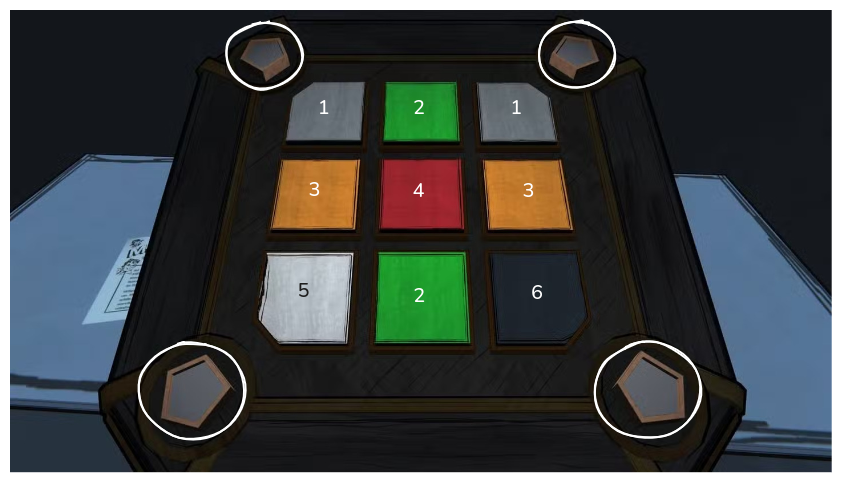
\includegraphics[scale=0.4]{imagens/caixa-mora-jai.png}
    \\\textbf{Fonte:} Adaptado de: \citeonline{polygon_mora_jai}
    \label{fig:caixa-mora-jai}
\end{figure}
\FloatBarrier

Observa-se na Figura \ref{fig:caixa-mora-jai} as seguintes peças e seus movimentos:

\begin{enumerate}
	\item Peças Cinzas: qualquer espaço com coloração cinza consiste da ausência de uma peça.
	\item Peças Verdes: se movimentam para o extremo oposto da sua posição atual. Isto é, caso haja uma peça verde no centro da linha do topo, ao clicar na peça, ela iria para o centro da linha do rodapé.
	\item Peças Laranjas: não possuem movimento algum, porém, são utilizadas, geralmente, como peças auxiliares para outras peças. Sua mecânica é a seguinte: caso uma peça laranja esteja cercada de duas ou mais peças de outra cor, a peça laranja, ao ser clicada, se torna desta cor.
	\item Peças Vermelhas: não possuem movimentação. Ao invés disso, ao clicar em uma peça vermelha, todas as peças brancas (5) se tornam peças pretas (6) e todas as peças pretas (6) se tornam peças vermelhas.
	\item Peças Brancas: se multiplicam para todos os espaços vazios adjacentes. Caso não haja espaços vazios, a peça branca clicada desaparece.
	\item Peças Pretas: se movimentam sempre para a direita, caso cheguem no final da linha voltam para o início.
\end{enumerate}

Além das peças, há também o objetivo de cada caixa. É possível observar na figura alguns símbolos nas quinas que foram circulados de branco. Cada símbolo indica qual peça precisa estar em cada uma das quinas. Os símbolos são baseados em reinos do jogo, onde cada reino possui uma cor que o representa. Neste caso, o jogador precisaria mover quatro peças vermelhas, a cor do reino de Fenn Aries, uma para cada quina.

\subsection{Conceitualização do Protótipo}

Dado tal contexto sobre as Caixas Mora Jai, o protótipo a ser desenvolvido será composto por quebra-cabeças onde cada nível possui uma grade de tamanhos variados. Assim como na inspiração, o protótipo também possuirá diversas peças com suas próprias movimentações e mecânicas. No entanto, para resolver o problema no qual pessoas daltônicas teriam ao brincar com Caixas Mora Jai todas as peças do protótipo possuirão, além de uma cor própria, um símbolo para representá-las.

\section{Definição de Escopo}

\subsection{Plataformas e Tecnologias}

Conforme citado anteriormente, o trabalho será feito com a ajuda da ferramenta de desenvolvimento de jogos Godot. Por conta disso, o protótipo final estará disponível para Computadores nos sistemas operacionais: Windows e Linux.

\subsection{Tamanho do Protótipo}

O Produto Mínimo Viável (MVP) deste trabalho terá uma duração curta. Inicialmente, pretende-se que sejam 15 níveis. Sendo divididos em três categorias:
\begin{itemize}
	\item 6 Níveis Introdutórios de Peças para apresentação das mecânicas de cada peça;
	\item 6 Níveis de Aprofundamento de Peças explorando as mecânicas de outras formas;
	\item 3 Níveis Finais contendo os principais desafios do jogo, contemplando tudo que foi aprendido até então.
\end{itemize}

No entanto, caso durante o desenvolvimento do protótipo novas ideias de peças ou níveis sejam concebidas, a dimensão do protótipo será devidamente ajustada para abranger o novo conteúdo.

O objetivo de cada nível introdutório do protótipo será, então: descobrir o movimento e mecânica das peças para poder movimentá-las para determinados cantos e poder solucionar o nível.

\subsection{Tema do Protótipo}

O tema principal do protótipo a ser desenvolvido serão animais. Cada peça será representada por um animal diferente como uma forma de indicar qual seria a movimentação daquela peça inspirada em seu animal de forma alegórica. Portanto, como o protótipo será envolto de animais e quebra-cabeças, o nome definido para chamá-lo será: Bicharada. O nome se trata, obviamente, de um trocadilho da palavra ``Bicharada'' que contém a palavra ``Charada'' em si.

\section{Estrutura do Protótipo}

Os tabuleiros do protótipo possuirão diferentes tamanhos para agregar a cada nível e seus respectivos desafios. Desta forma, a seguir, na Figura \ref{fig:tabuleiros-bicharada} pode-se observar quais serão os diferentes tamanhos de tabuleiro que estarão no protótipo.

\begin{figure}[!htbp]
    \centering
    \caption{Exemplos de Tabuleiros do Bicharada}
    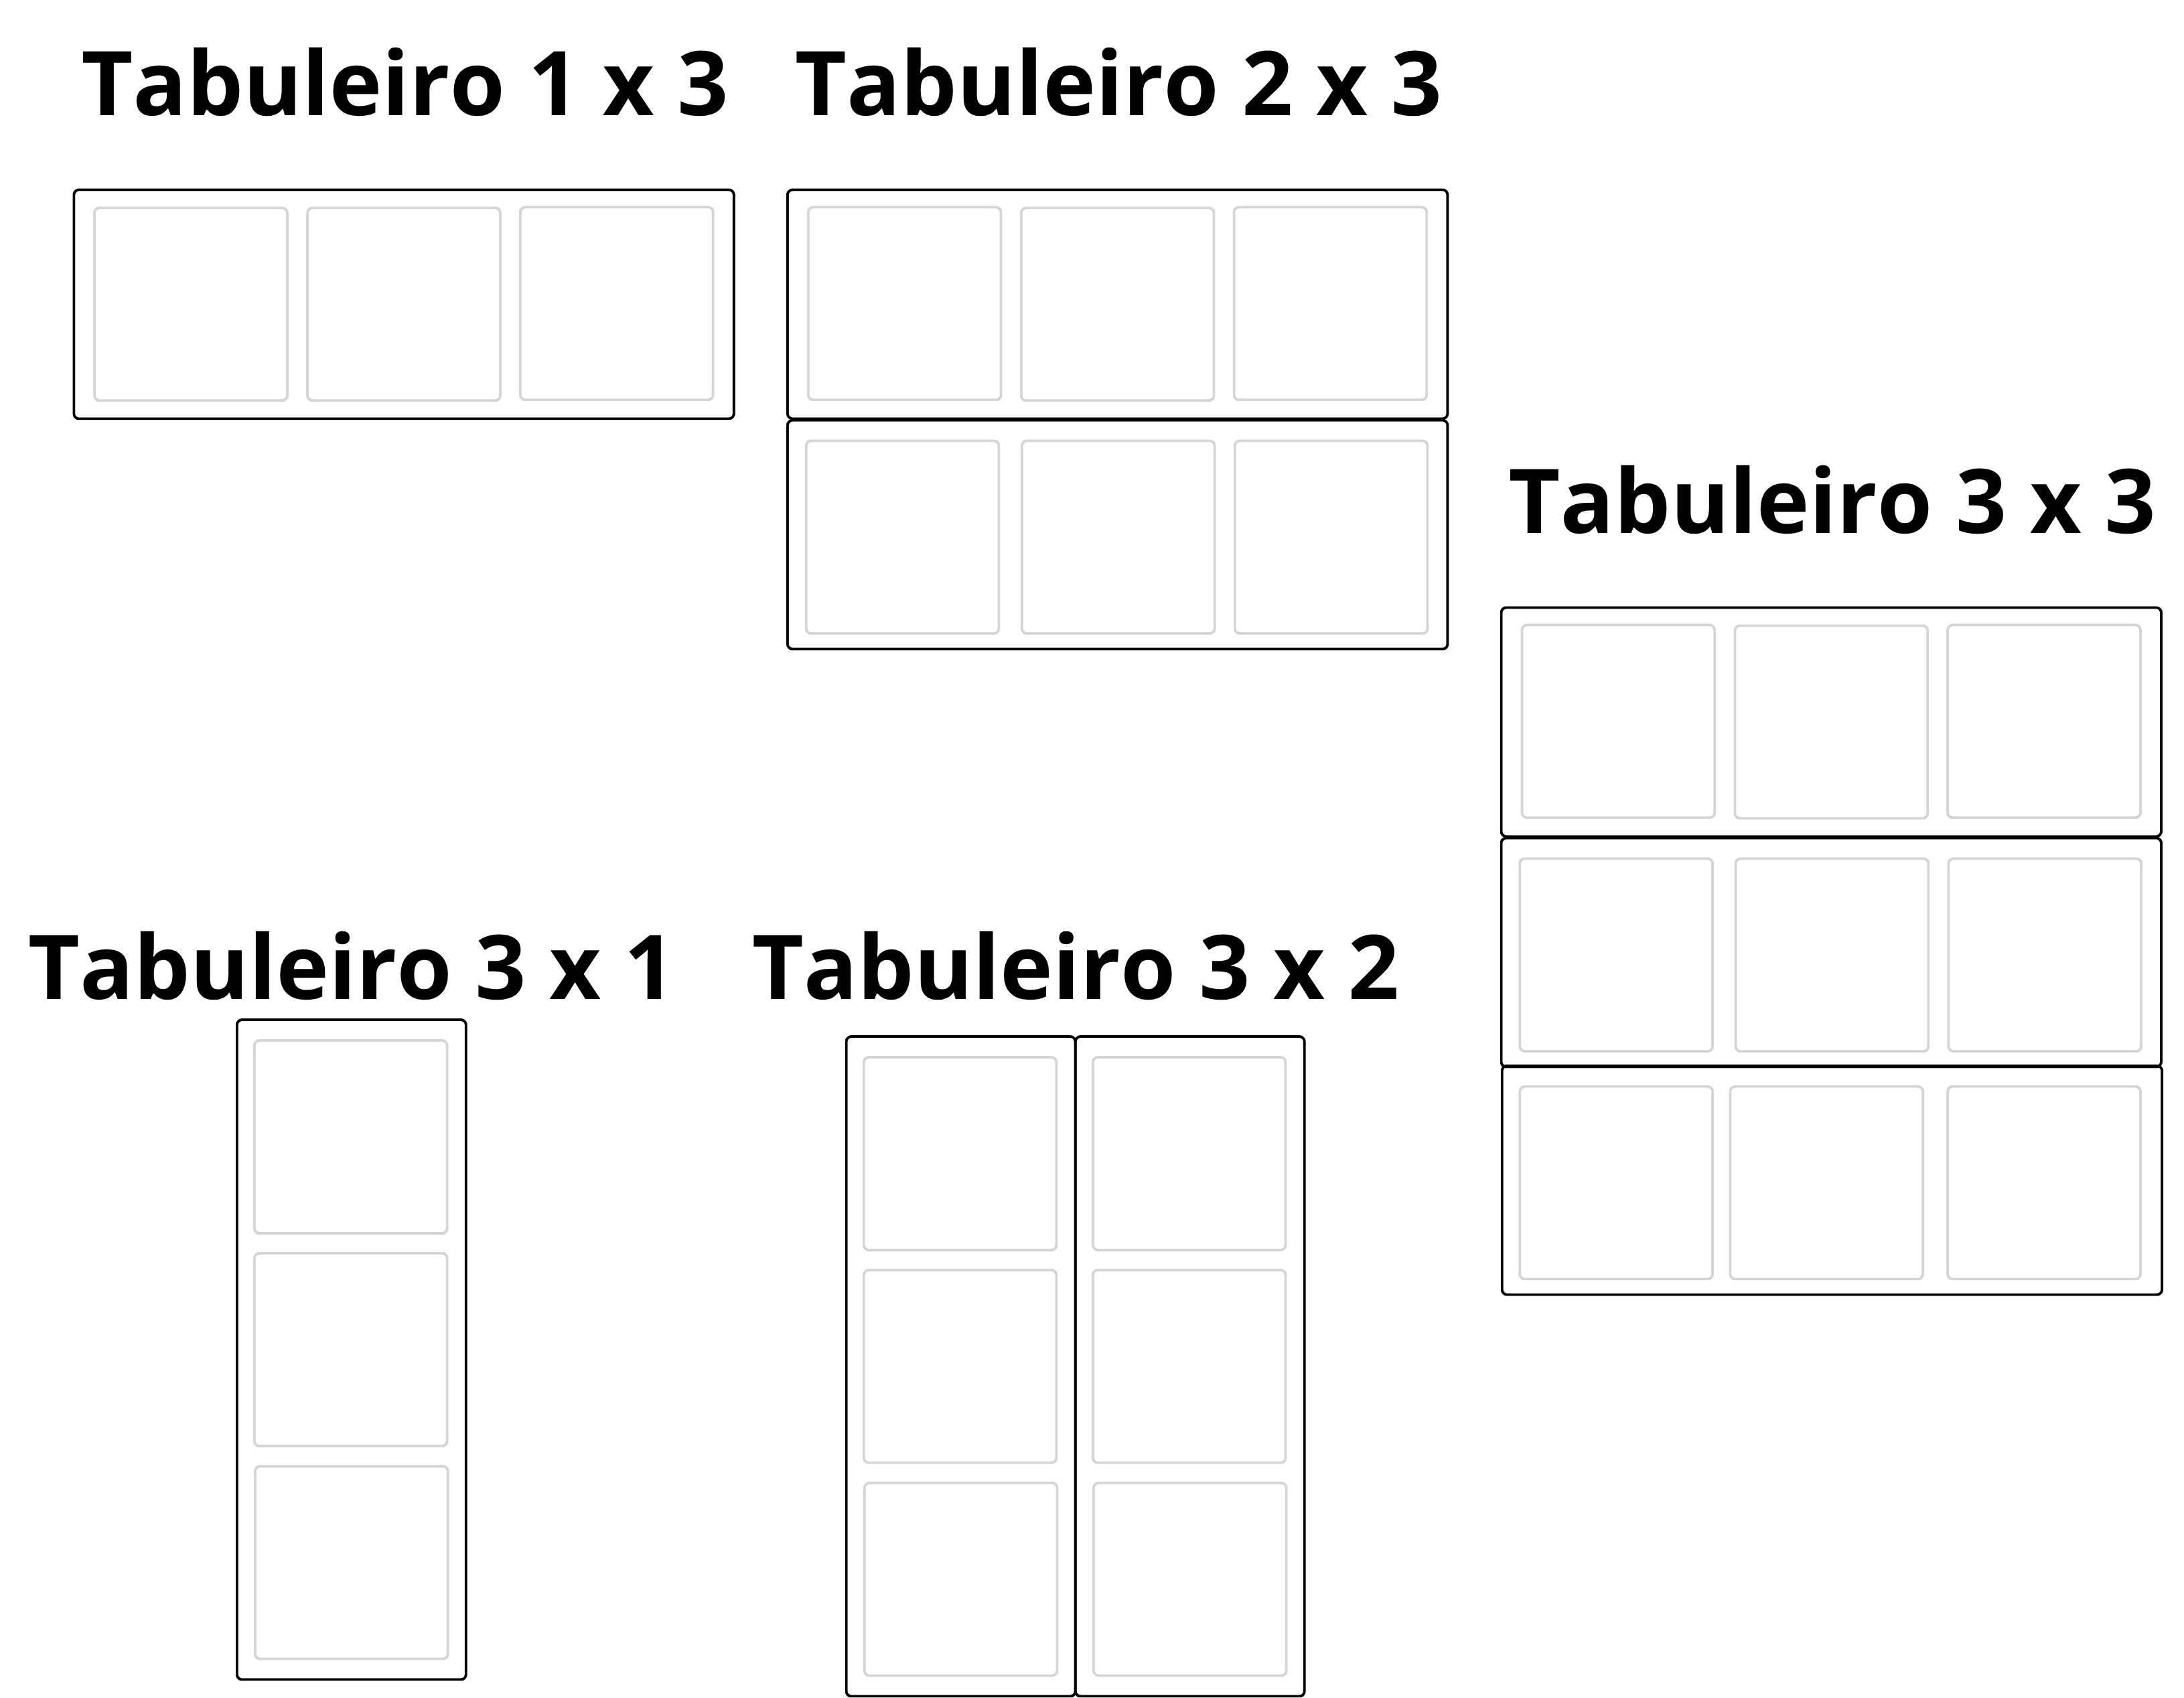
\includegraphics[scale=0.12]{imagens/tabuleiros-bicharada.png}
    \\\textbf{Fonte:} Elaborado pelo Autor
    \label{fig:tabuleiros-bicharada}
\end{figure}
\FloatBarrier

Os níveis do protótipo possuirão os seguintes elementos:

\begin{itemize}
	\item Um tabuleiro;
	\item Uma ou mais peças;
	\item Um ou mais círculos com ícone que representará alguma das peças existentes no nível.
\end{itemize}

A seguir, observa-se na Figura \ref{fig:exemplo-nivel-bicharada} um nível contendo:

\begin{itemize}
	\item Um tabuleiro de tamanho 1 × 3;
	\item Uma peça de Rato;
	\item Um círculo com o ícone do Rato.
\end{itemize}


\begin{figure}[!htbp]
    \centering
    \caption{Exemplo de Nível do Bicharada}
    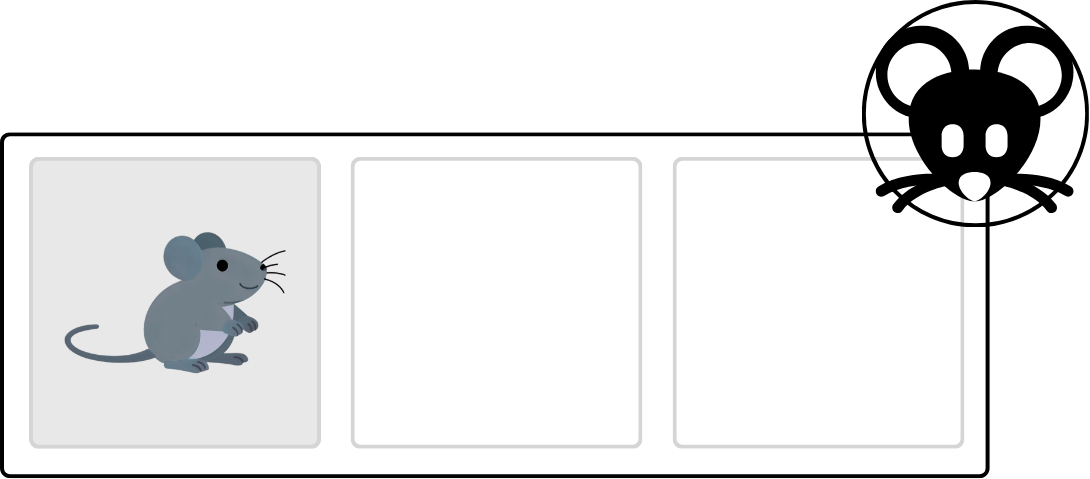
\includegraphics[scale=0.4]{imagens/exemplo-nível-bicharada.png}
    \\\textbf{Fonte:} Elaborado pelo Autor
    \label{fig:exemplo-nivel-bicharada}
\end{figure}
\FloatBarrier

Desta forma, o objetivo do jogador neste nível seria: movimentar a peça do Rato até o canto direito do tabuleiro, onde há o círculo com ícone do Rato.

Todos os níveis possuirão esta estrutura de movimentar diferentes peças para diferentes células do tabuleiro.

\subsection{Peças do Protótipo}

Definido então o tema, escopo e estrutura do Bicharada, a seguir serão descritas cada uma das peças que existirão no protótipo: 

\subsubsection{Rato}

A peça do Rato será de uma cor acinzentada, contendo o desenho de um rato. Ao ser clicado, o Rato se movimenta sempre para a direita. 
Caso esteja no final de uma linha, o Rato ignora a parede da direita e volta para o começo da linha.
Quando o Rato está à esquerda de outra peça, ao ser clicado, o Rato e a peça trocam de posições.

O nível introdutório do Rato, além da forma de como resolvê-lo, pode ser observado na Figura \ref{fig:rascunho-nivel-introdutorio-rato}.

\begin{figure}[!htbp]
    \centering
    \caption{Rascunho do Nível Introdutório da Peça Rato}
    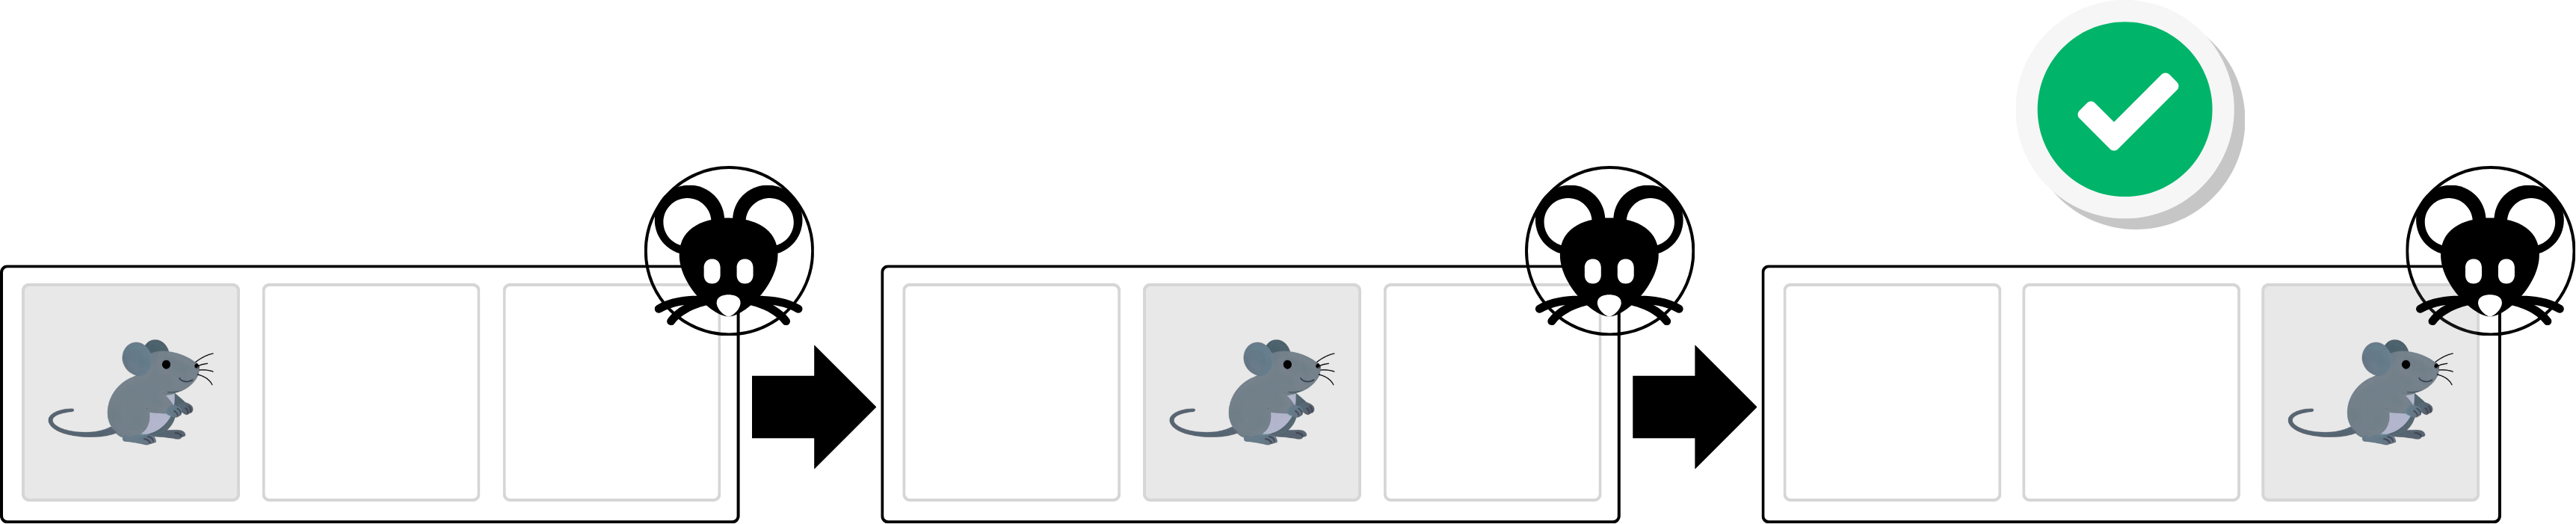
\includegraphics[scale=0.15]{imagens/nivel-introdutorio-rato.png}
    \\\textbf{Fonte:} Elaborado pelo Autor
    \label{fig:rascunho-nivel-introdutorio-rato}
\end{figure}
\FloatBarrier

Este será o primeiro nível do protótipo, almeja-se a introdução do jogo não só como uma peça com movimentação simples, mas também com um conceito simples: o jogador clica na peça do Rato, e então percebe que o mesmo se movimenta para direita e desta forma consegue resolver o nível facilmente.

\begin{figure}[!htbp]
    \centering
    \caption{Rascunho do Nível de Aprofundamento da Peça Rato}
    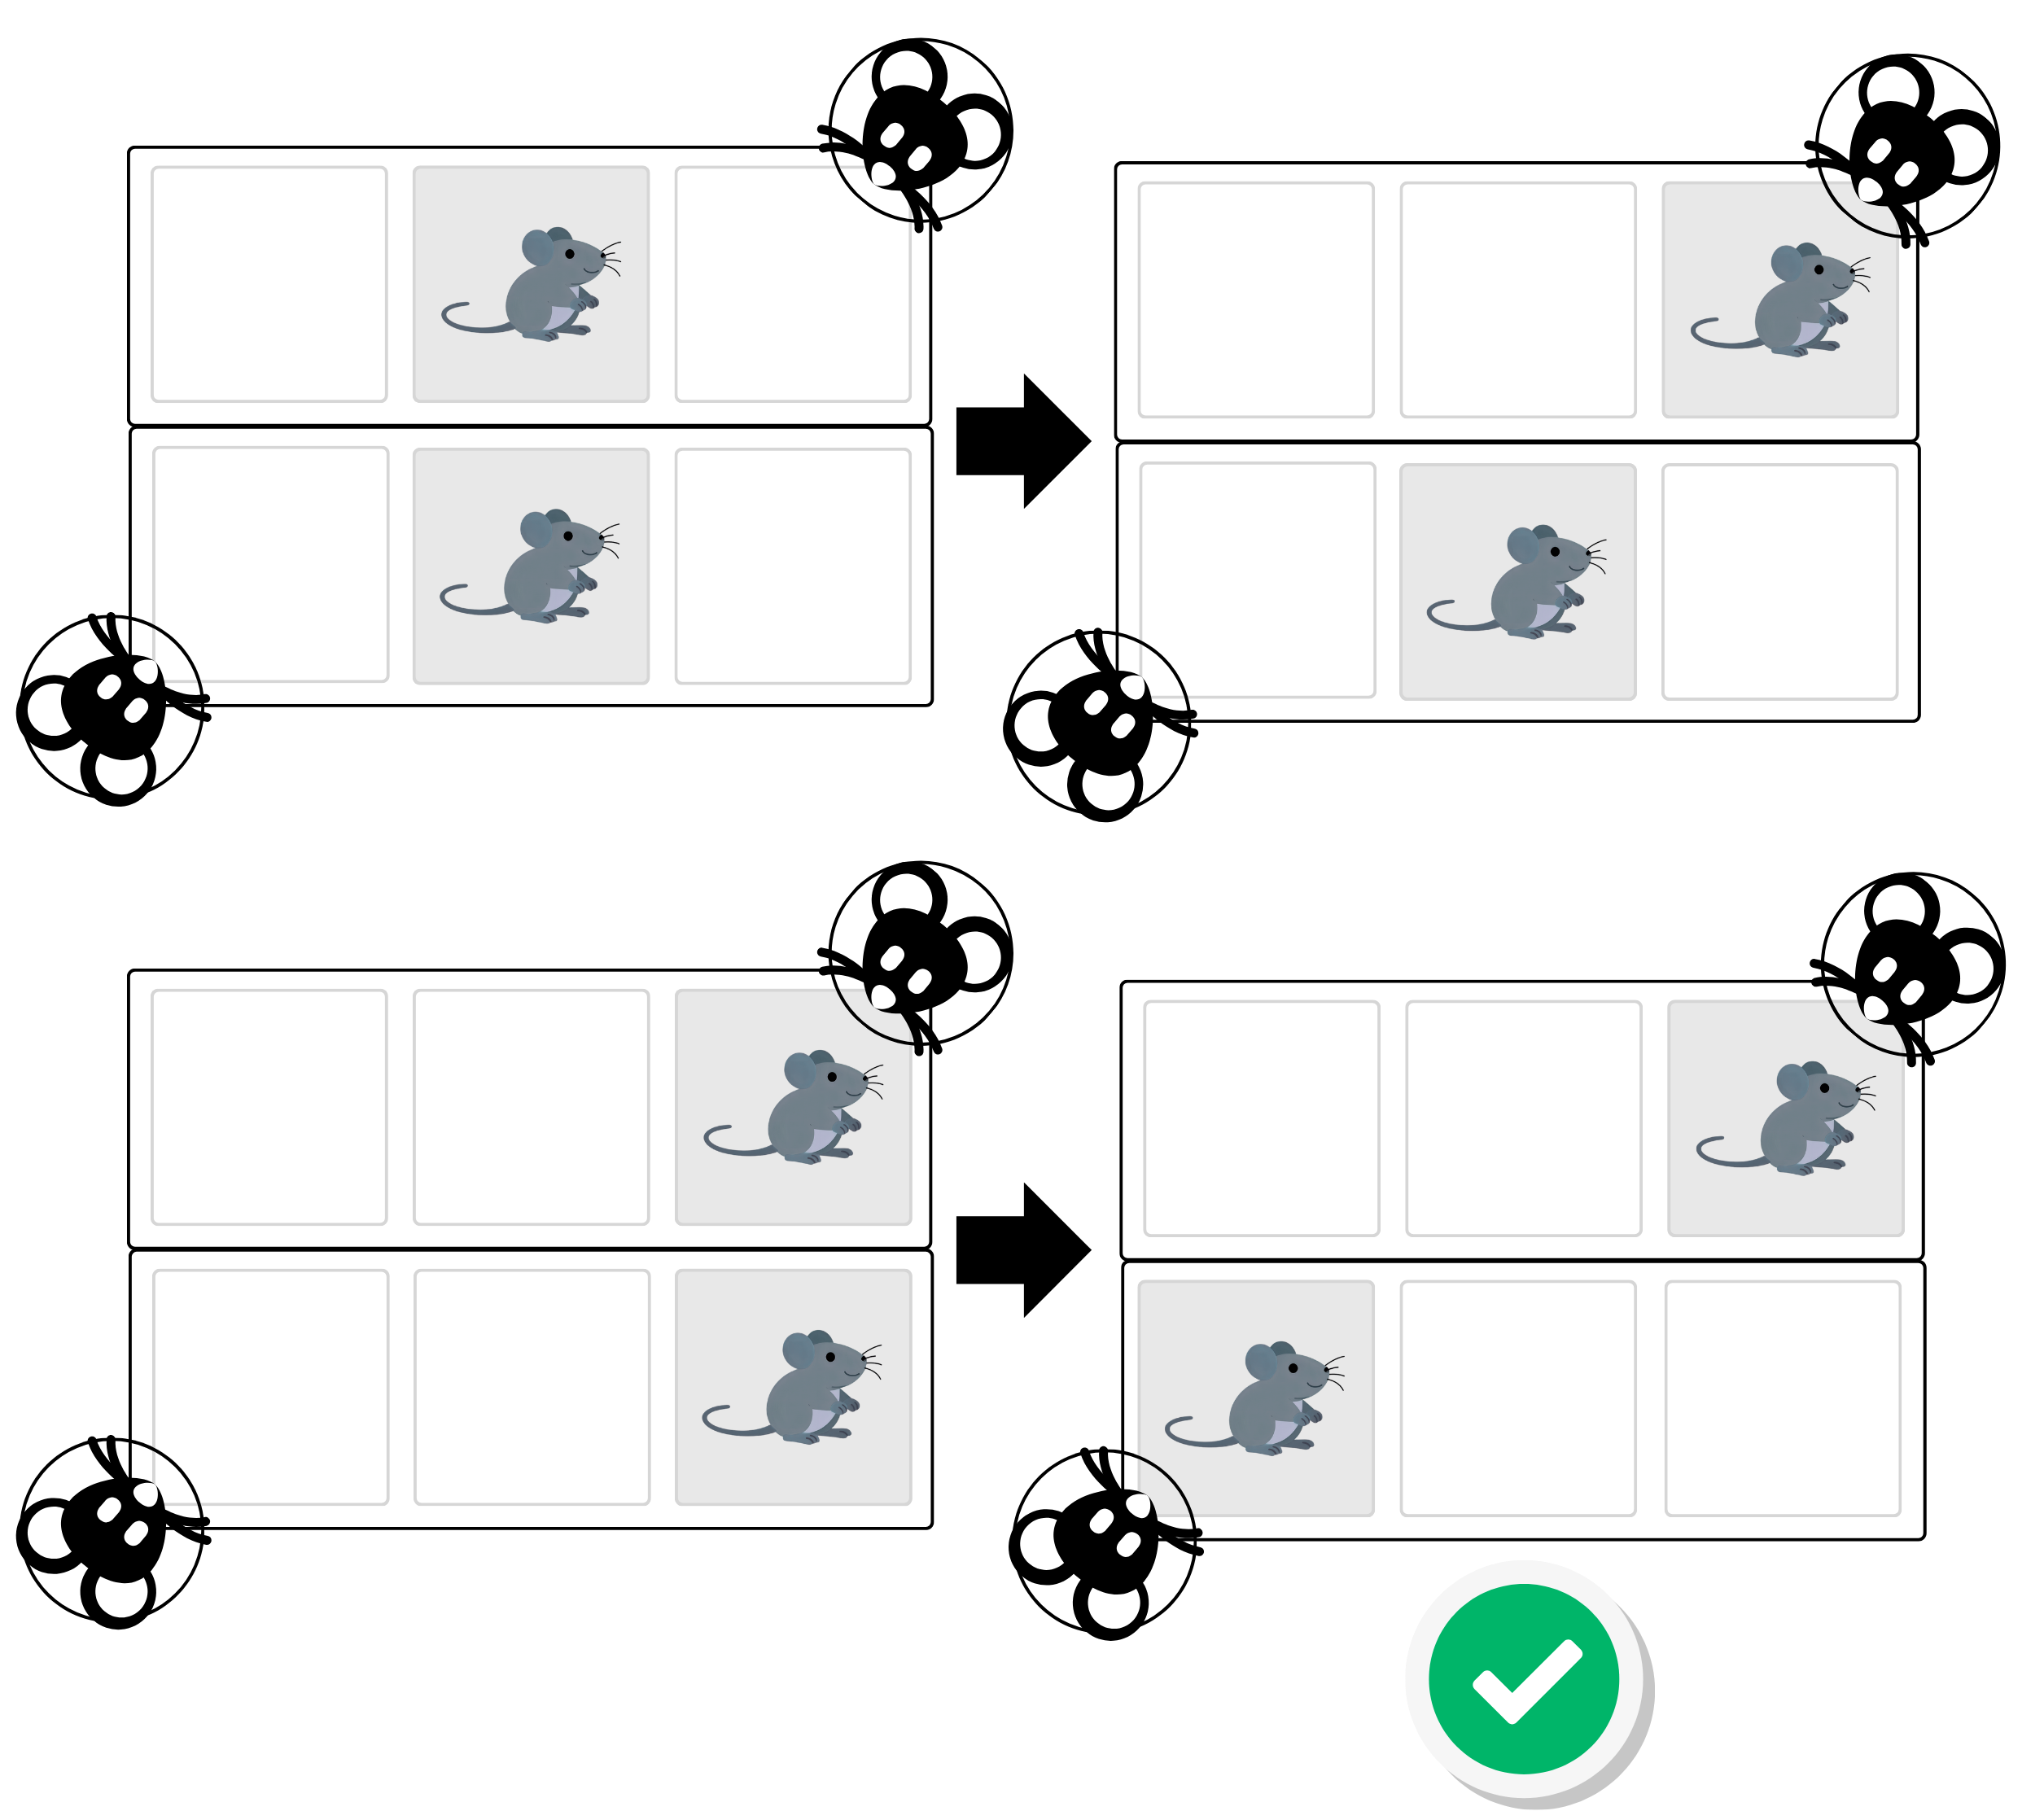
\includegraphics[scale=0.18]{imagens/nivel-aprofundamento-rato.png}
    \\\textbf{Fonte:} Elaborado pelo Autor
    \label{fig:rascunho-nivel-aprofundamento-rato}
\end{figure}
\FloatBarrier

O nível de aprofundamento do Rato possui como objetivo ensinar ao jogador a mecânica do Rato de ignorar a parede da direita e voltar para o começo da linha.
Observa-se na Figura \ref{fig:rascunho-nivel-aprofundamento-rato} o planejamento deste nível.

\subsubsection{Baleia}

A peça da Baleia possuirá uma cor azulada, contendo o desenho de uma baleia. Ao ser clicada, a Baleia se movimenta sempre para baixo. Quando a Baleia está logo acima de uma peça, ao ser clicada, a Baleia e a peça trocam de posições. 
Ex: Baleia acima de um Rato. Ao clicar na Baleia, o Rato iria para cima da Baleia.

\begin{figure}[!htbp]
    \centering
    \caption{Rascunho do Nível Introdutório da Peça Baleia}
    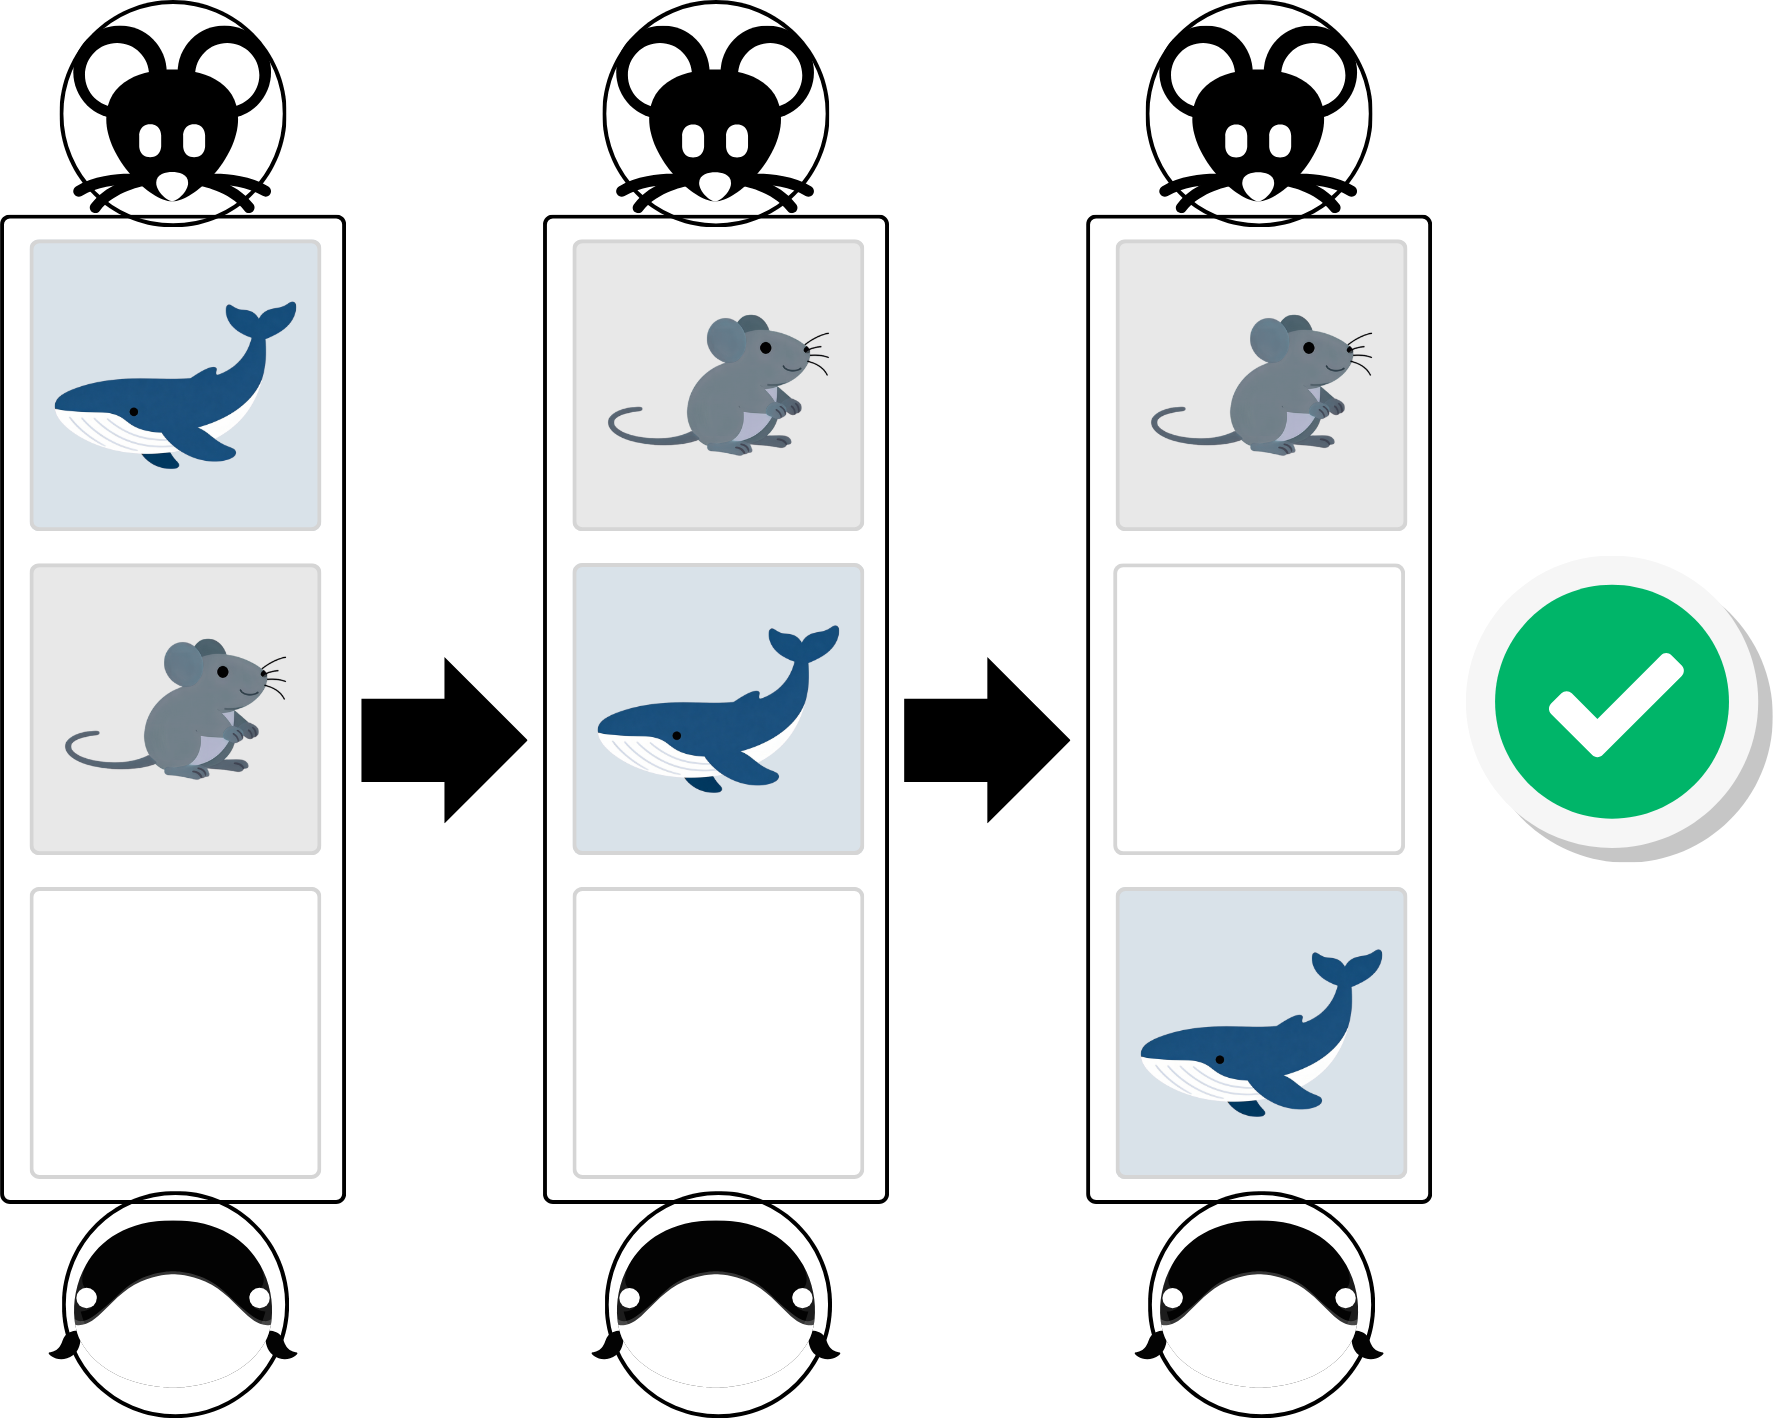
\includegraphics[scale=0.15]{imagens/nivel-introdutorio-baleia.png}
    \\\textbf{Fonte:} Elaborado pelo Autor
    \label{fig:rascunho-nivel-introdutorio-baleia}
\end{figure}
\FloatBarrier

\begin{figure}[!htbp]
    \centering
    \caption{Rascunho do Nível de Aprofundamento da Peça Baleia}
    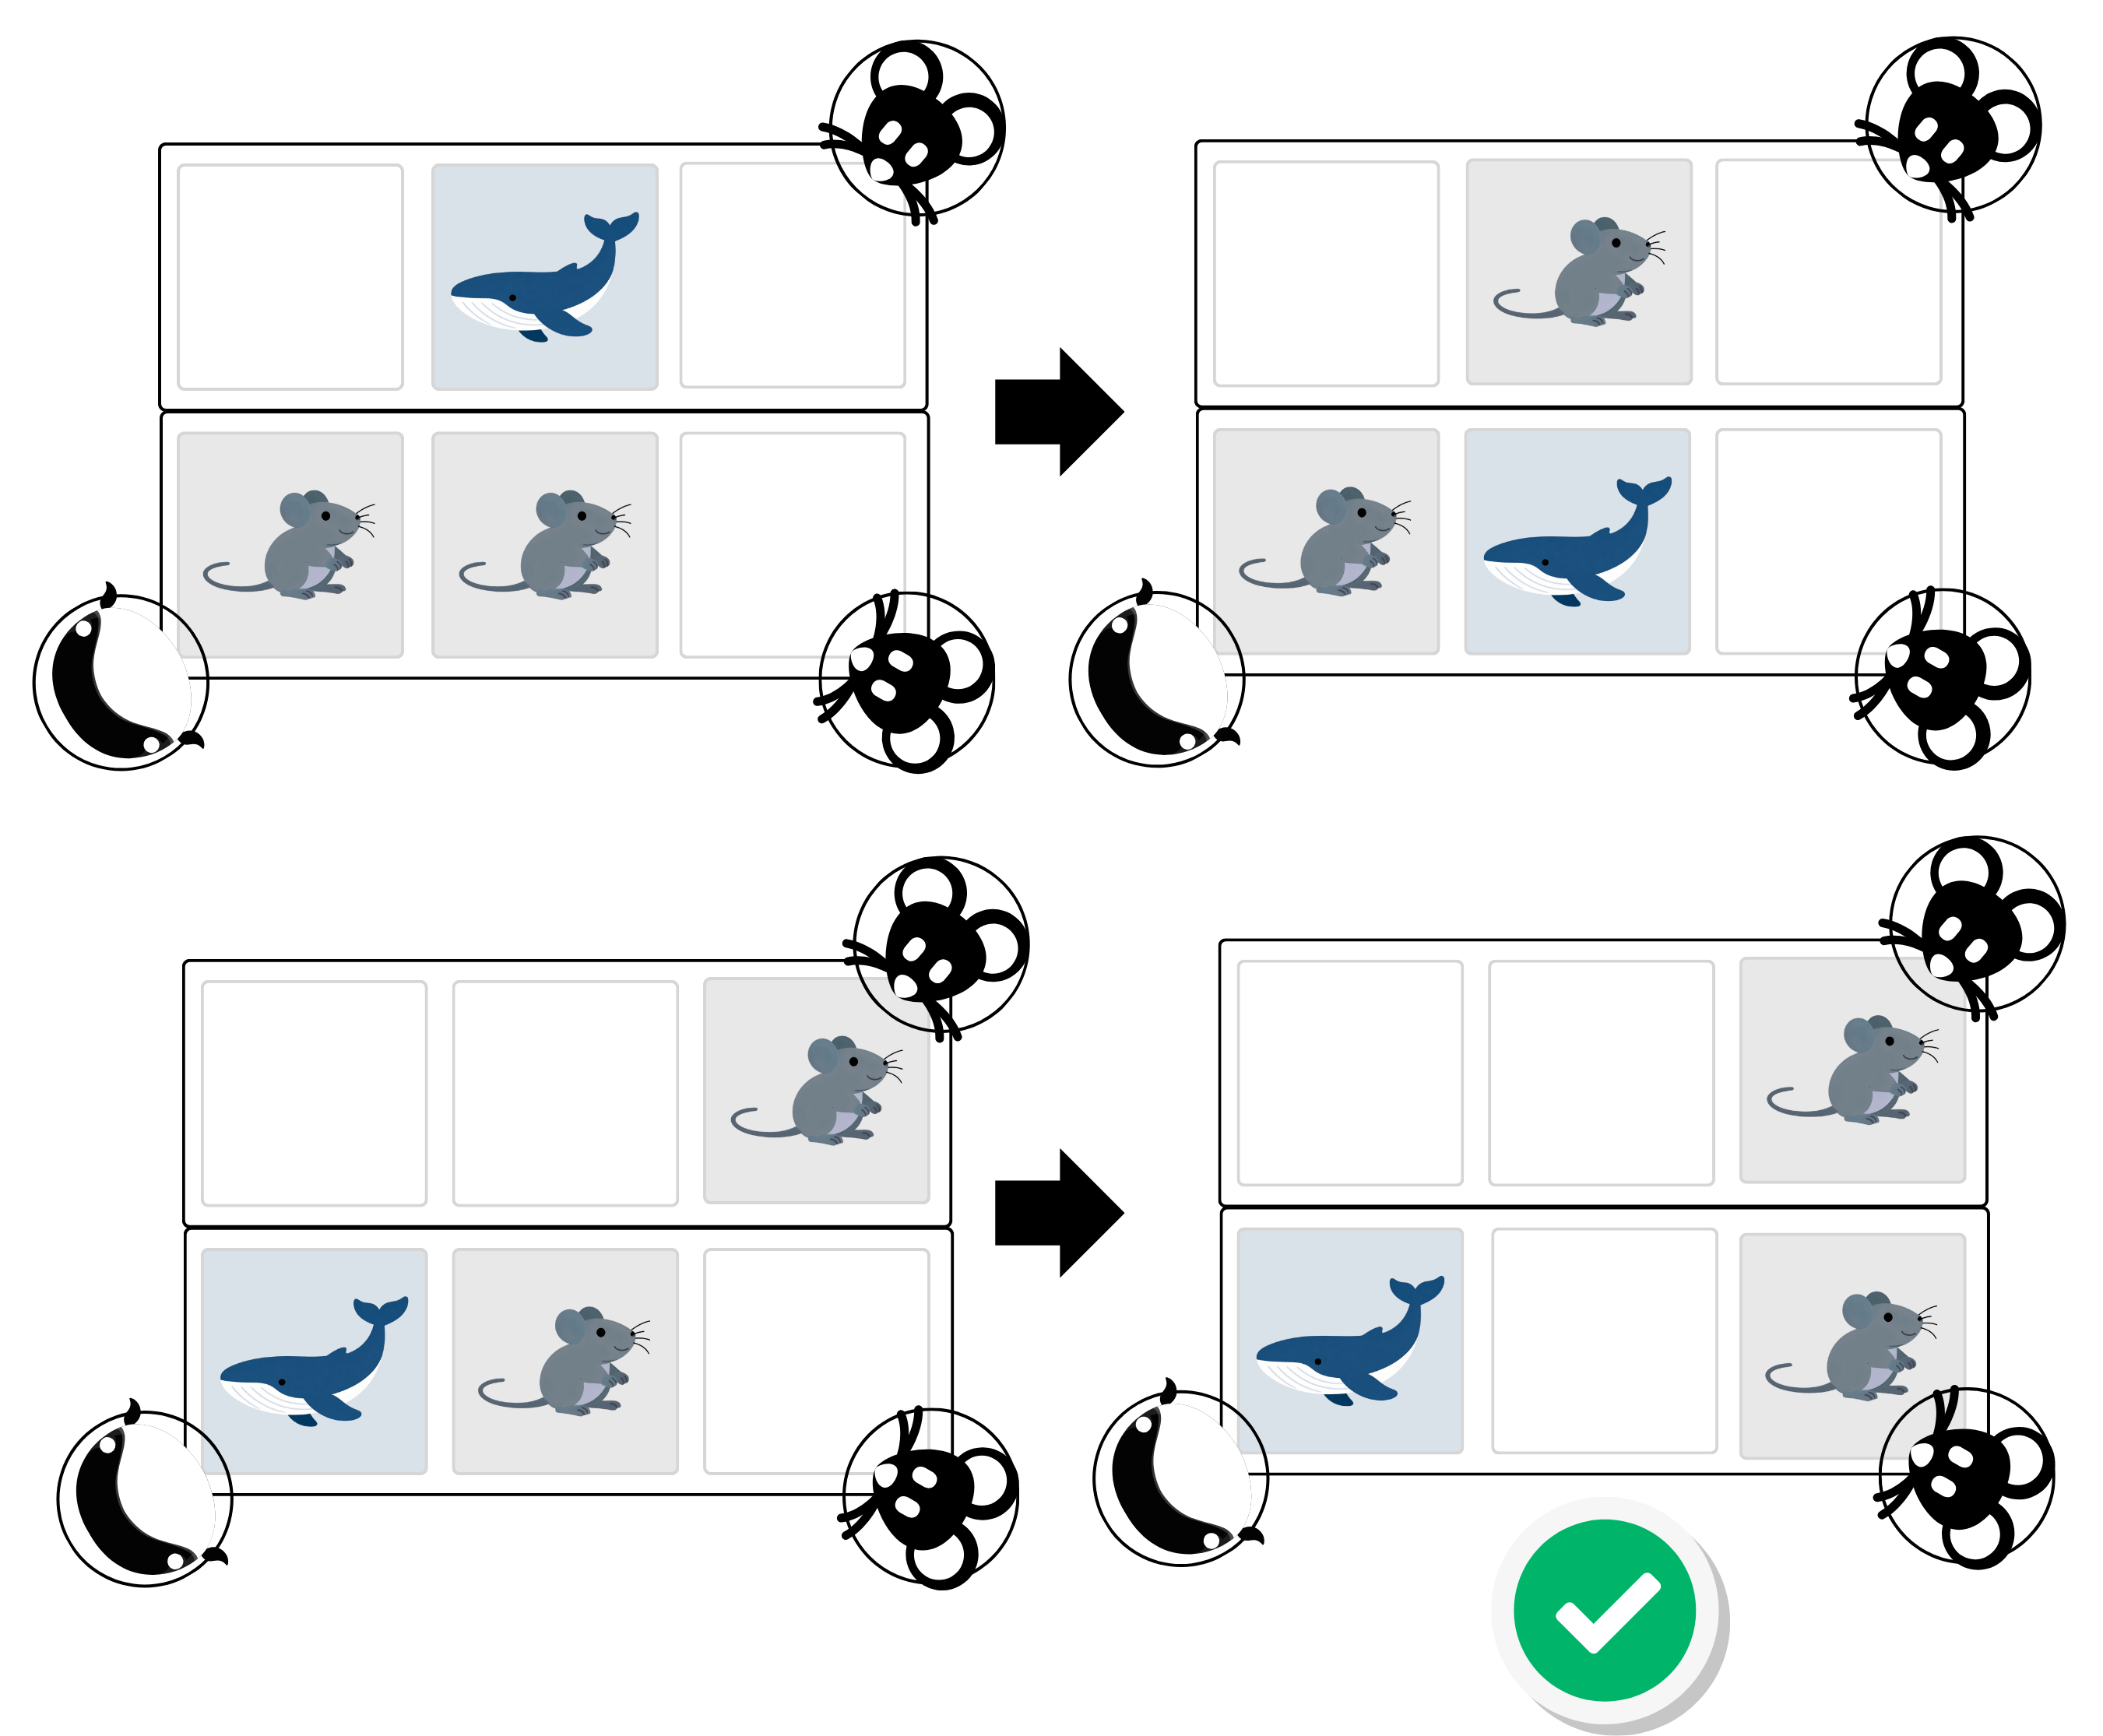
\includegraphics[scale=0.18]{imagens/nivel-aprofundamento-baleia.png}
    \\\textbf{Fonte:} Elaborado pelo Autor
    \label{fig:rascunho-nivel-aprofundamento-baleia}
\end{figure}
\FloatBarrier

Aqui não terminei de escrever ainda.

\subsubsection{Macaco}

A peça do Macaco possuirá uma cor amarronzada, contendo o desenho de um macaco. Ao ser clicado, se movimenta sempre para cima. Quando o Macaco está logo acima de uma peça, ao ser clicado, o Macaco e a peça trocam de posições. 
Ex: Macaco abaixo de um Rato. Ao clicar no Macaco, o Macaco iria para cima do Rato.

\begin{figure}[!htbp]
    \centering
    \caption{Rascunho do Nível Introdutório da Peça Macaco}
    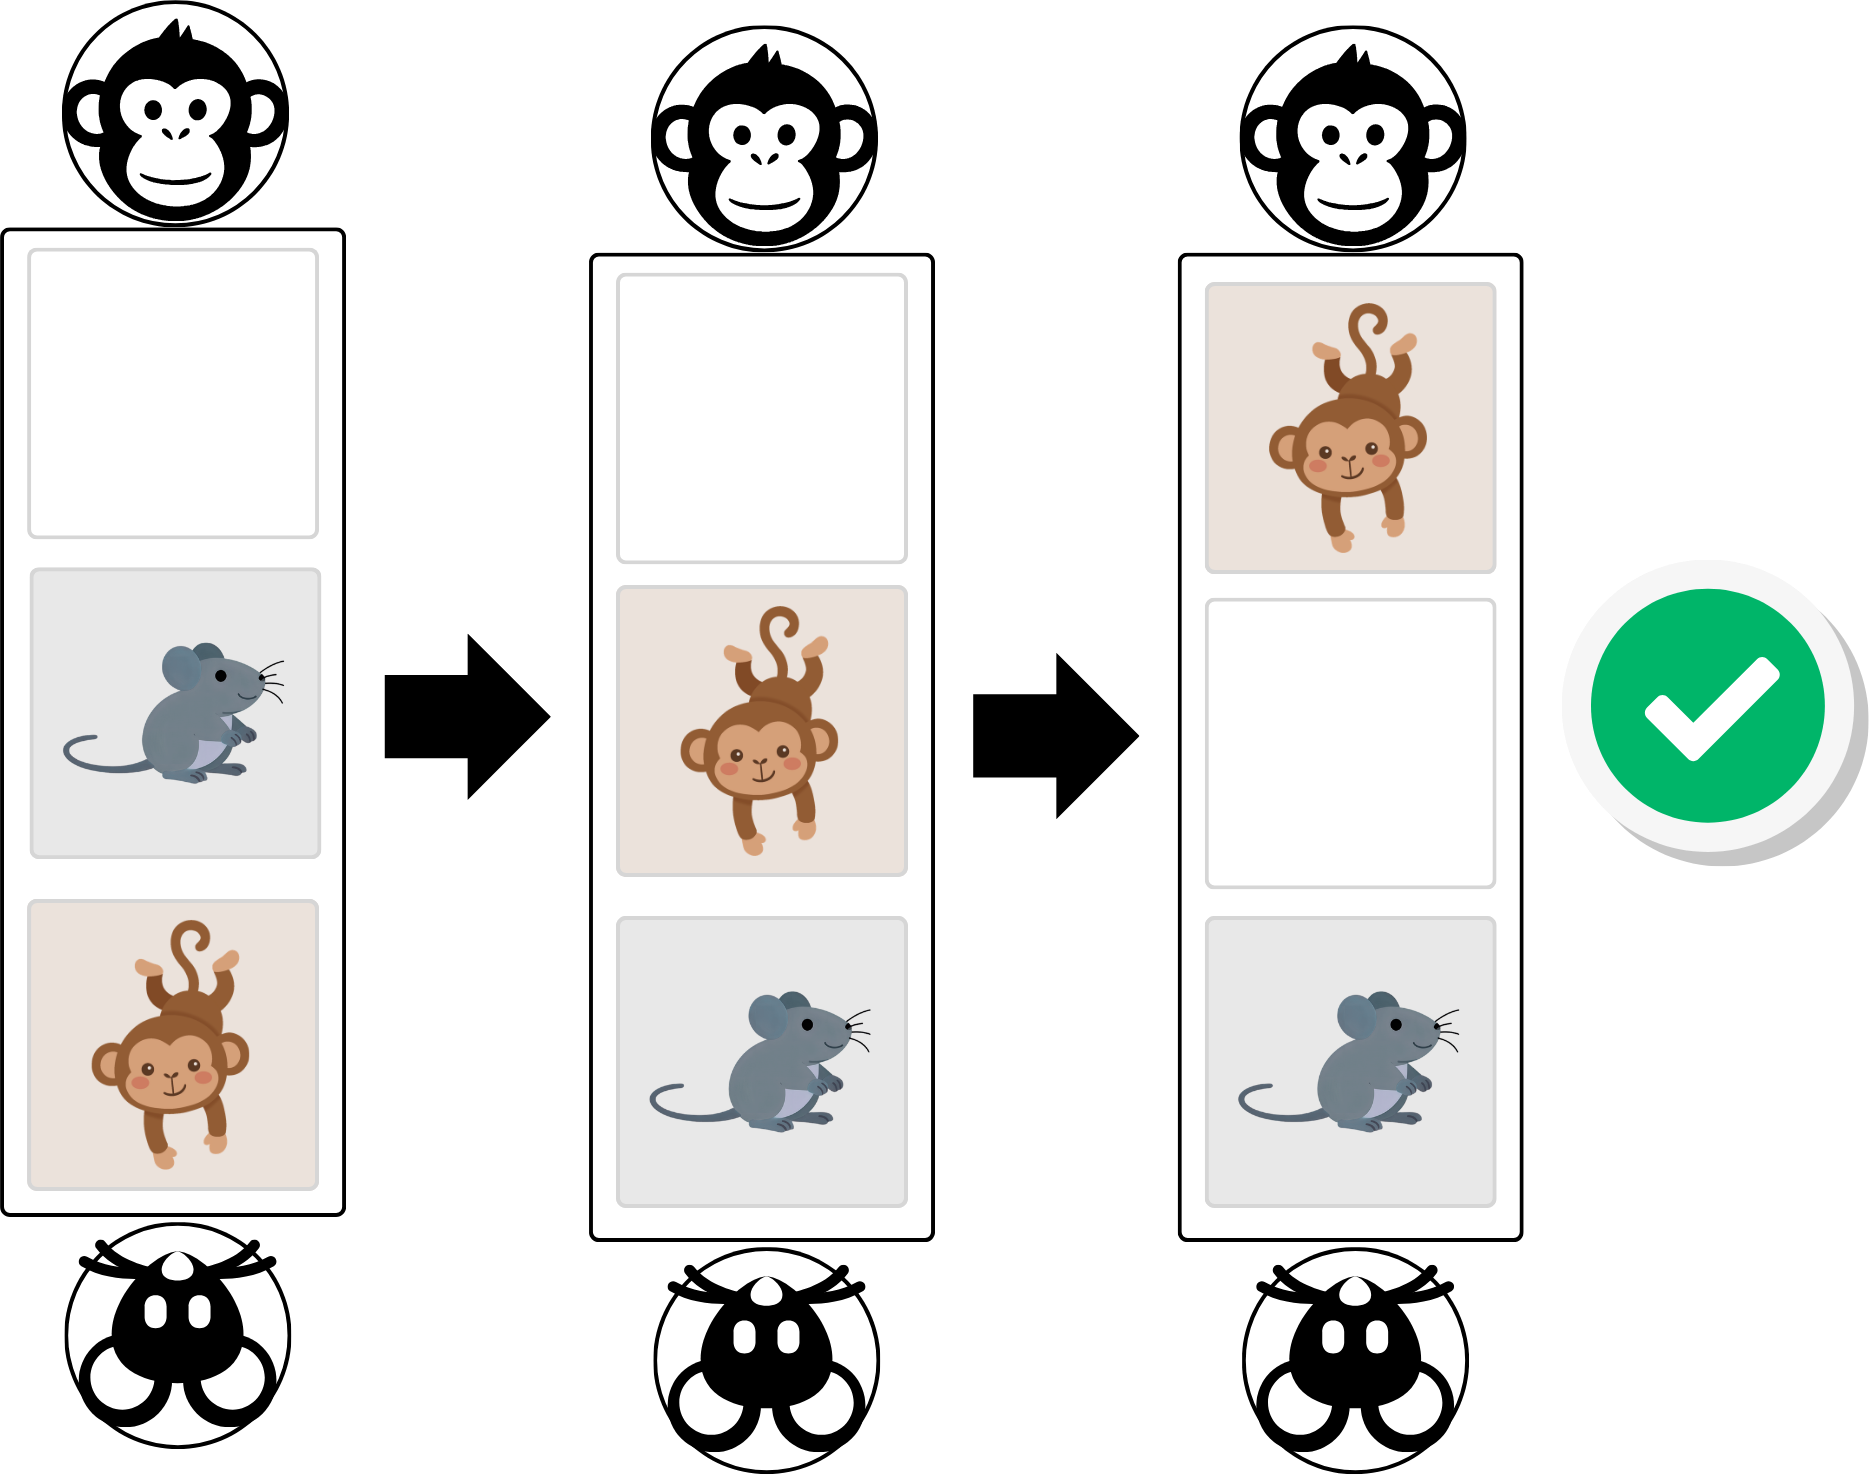
\includegraphics[scale=0.15]{imagens/nivel-introdutorio-macaco.png}
    \\\textbf{Fonte:} Elaborado pelo Autor
    \label{fig:rascunho-nivel-introdutorio-macaco}
\end{figure}
\FloatBarrier

\begin{figure}[!htbp]
    \centering
    \caption{Rascunho do Nível de Aprofundamento da Peça Macaco}
    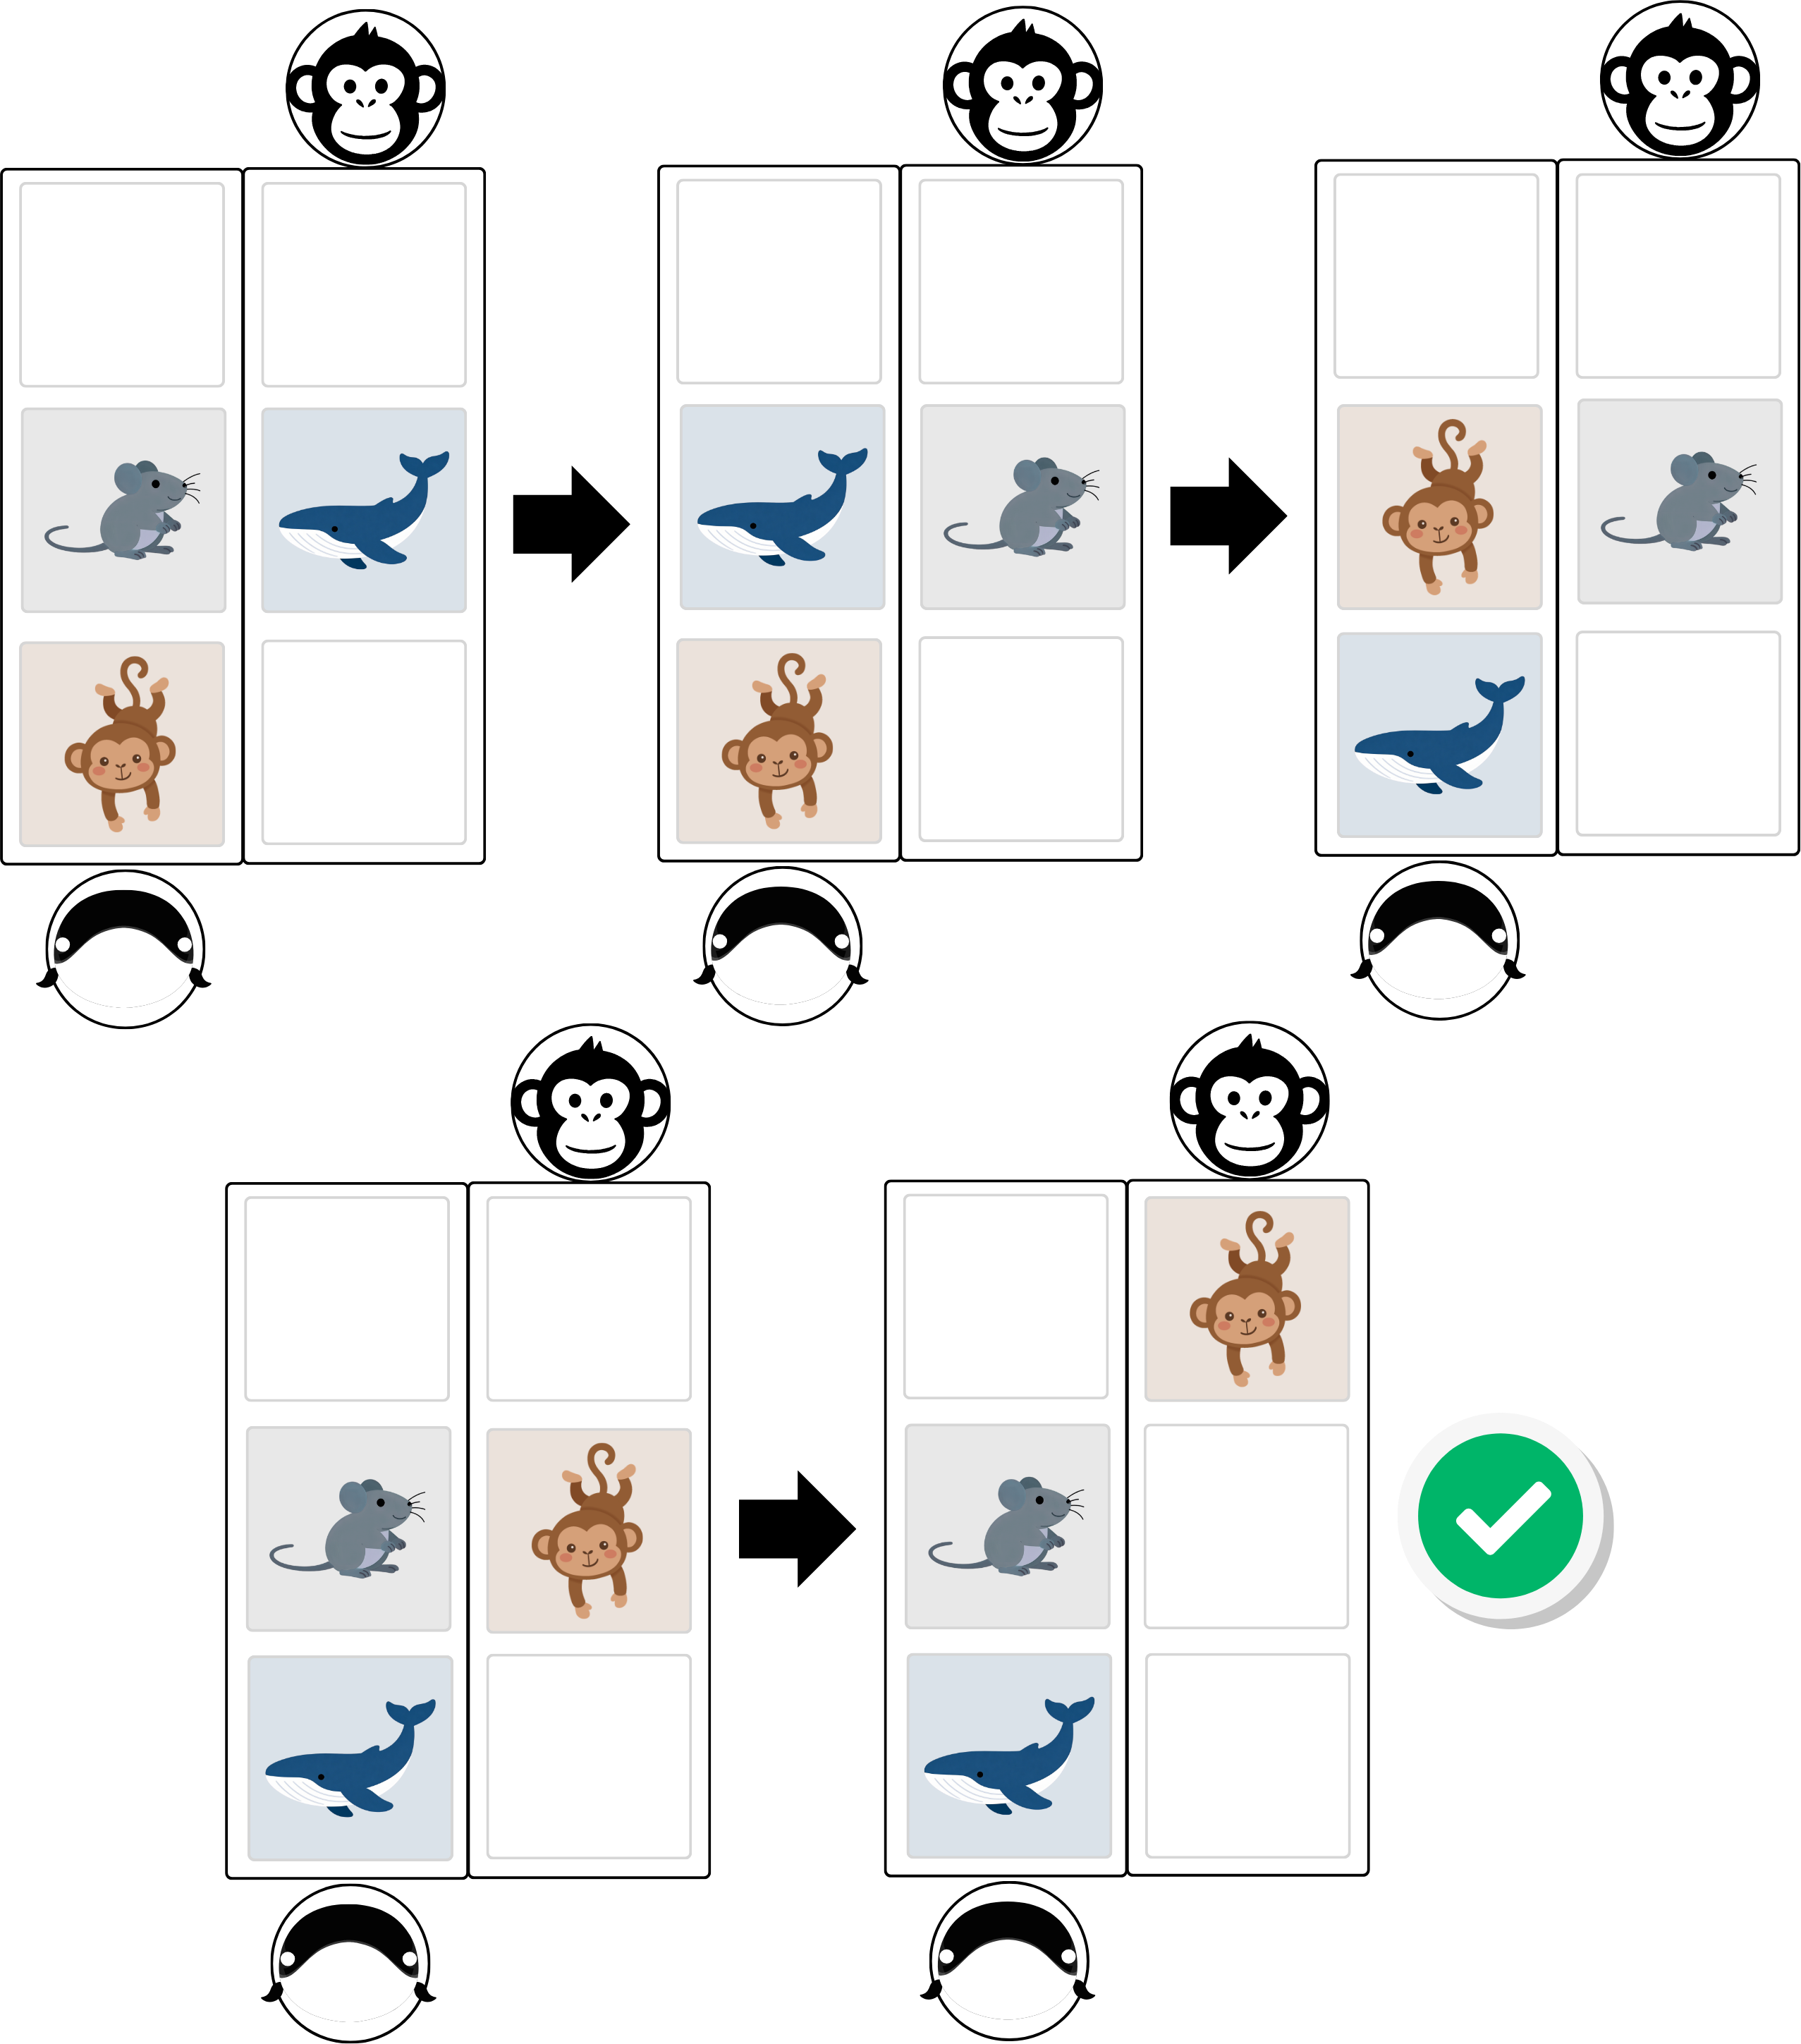
\includegraphics[scale=0.18]{imagens/nivel-aprofundamento-macaco.png}
    \\\textbf{Fonte:} Elaborado pelo Autor
    \label{fig:rascunho-nivel-aprofundamento-macaco}
\end{figure}
\FloatBarrier

Aqui não terminei de escrever ainda.

\subsubsection{Camaleão}

A peça do Camaleão possuirá uma cor esverdeada, contendo o desenho de um camaleão. Esta peça existirá somente em tabuleiros 3 × 3. Sua movimentação espelha a movimentação da peça que estiver no centro do tabuleiro na posição (2,2). Copia todos os trejeitos da peça que estiver no centro.

\begin{figure}[!htbp]
    \centering
    \caption{Rascunho do Nível Introdutório da Peça Camaleão}
    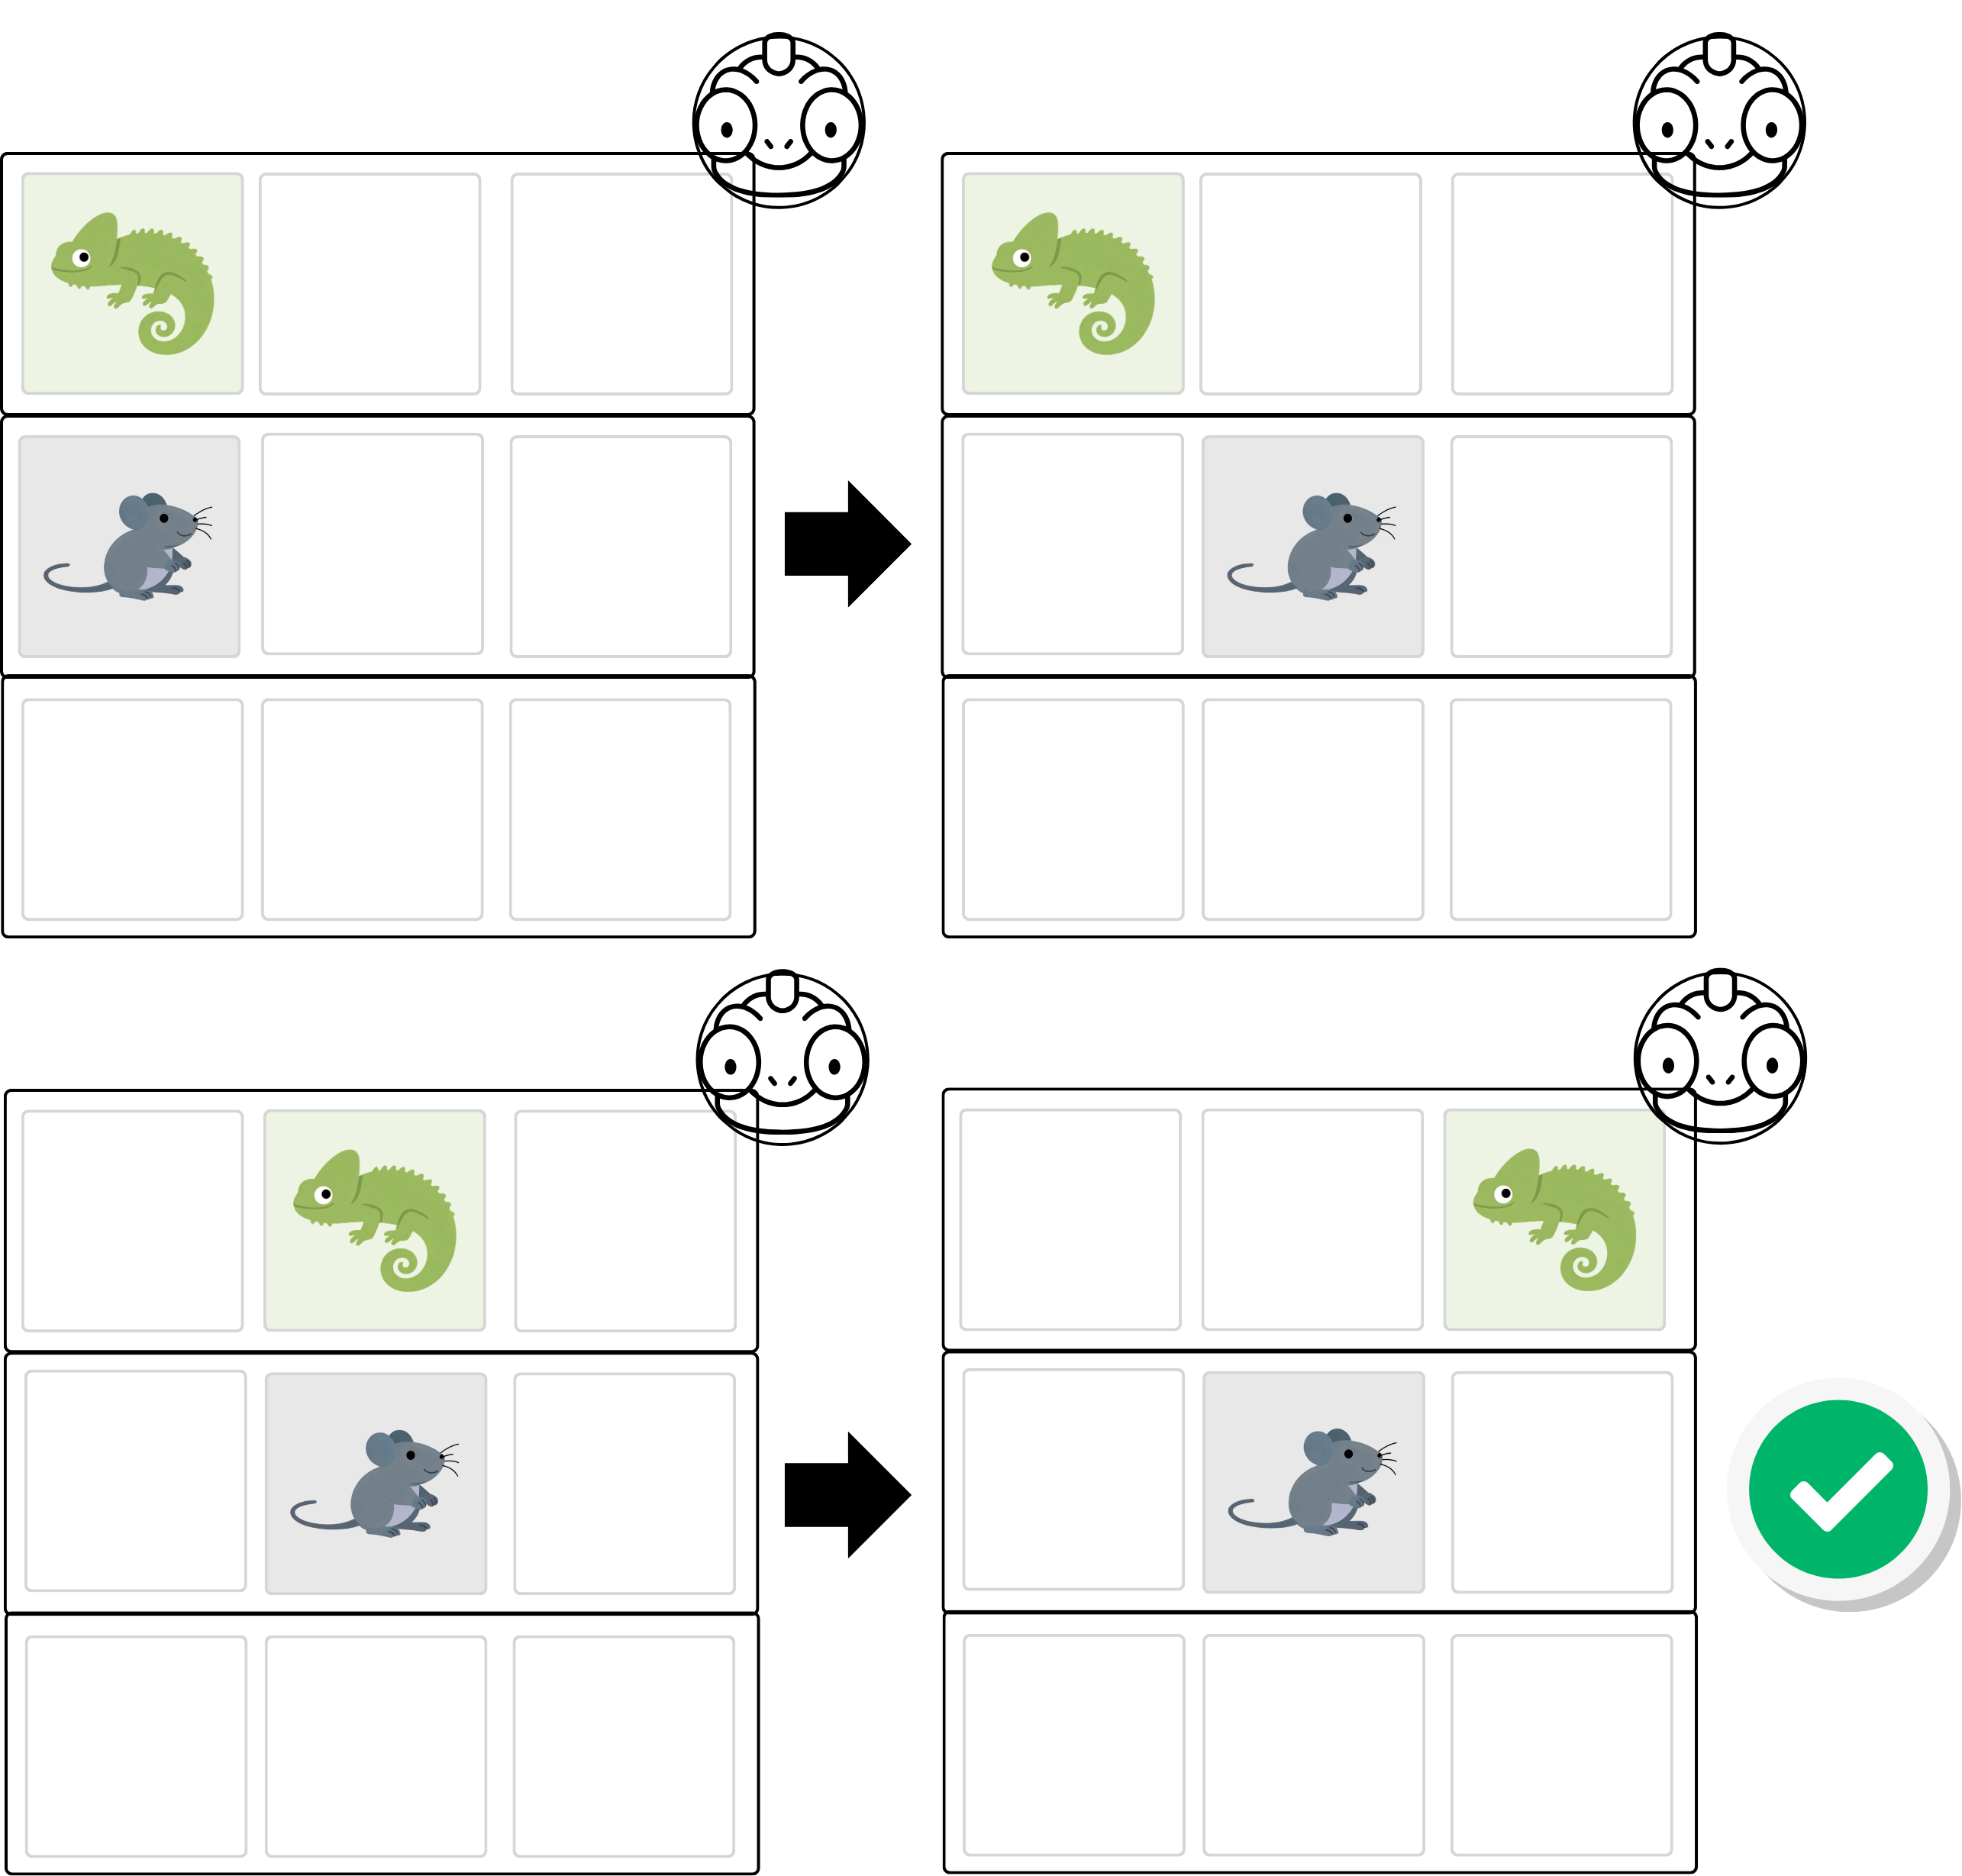
\includegraphics[scale=0.15]{imagens/nivel-introdutorio-camaleao.png}
    \\\textbf{Fonte:} Elaborado pelo Autor
    \label{fig:rascunho-nivel-introdutorio-camaleao}
\end{figure}
\FloatBarrier

\begin{figure}[!htbp]
    \centering
    \caption{Rascunho do Nível de Aprofundamento da Peça Camaleão}
    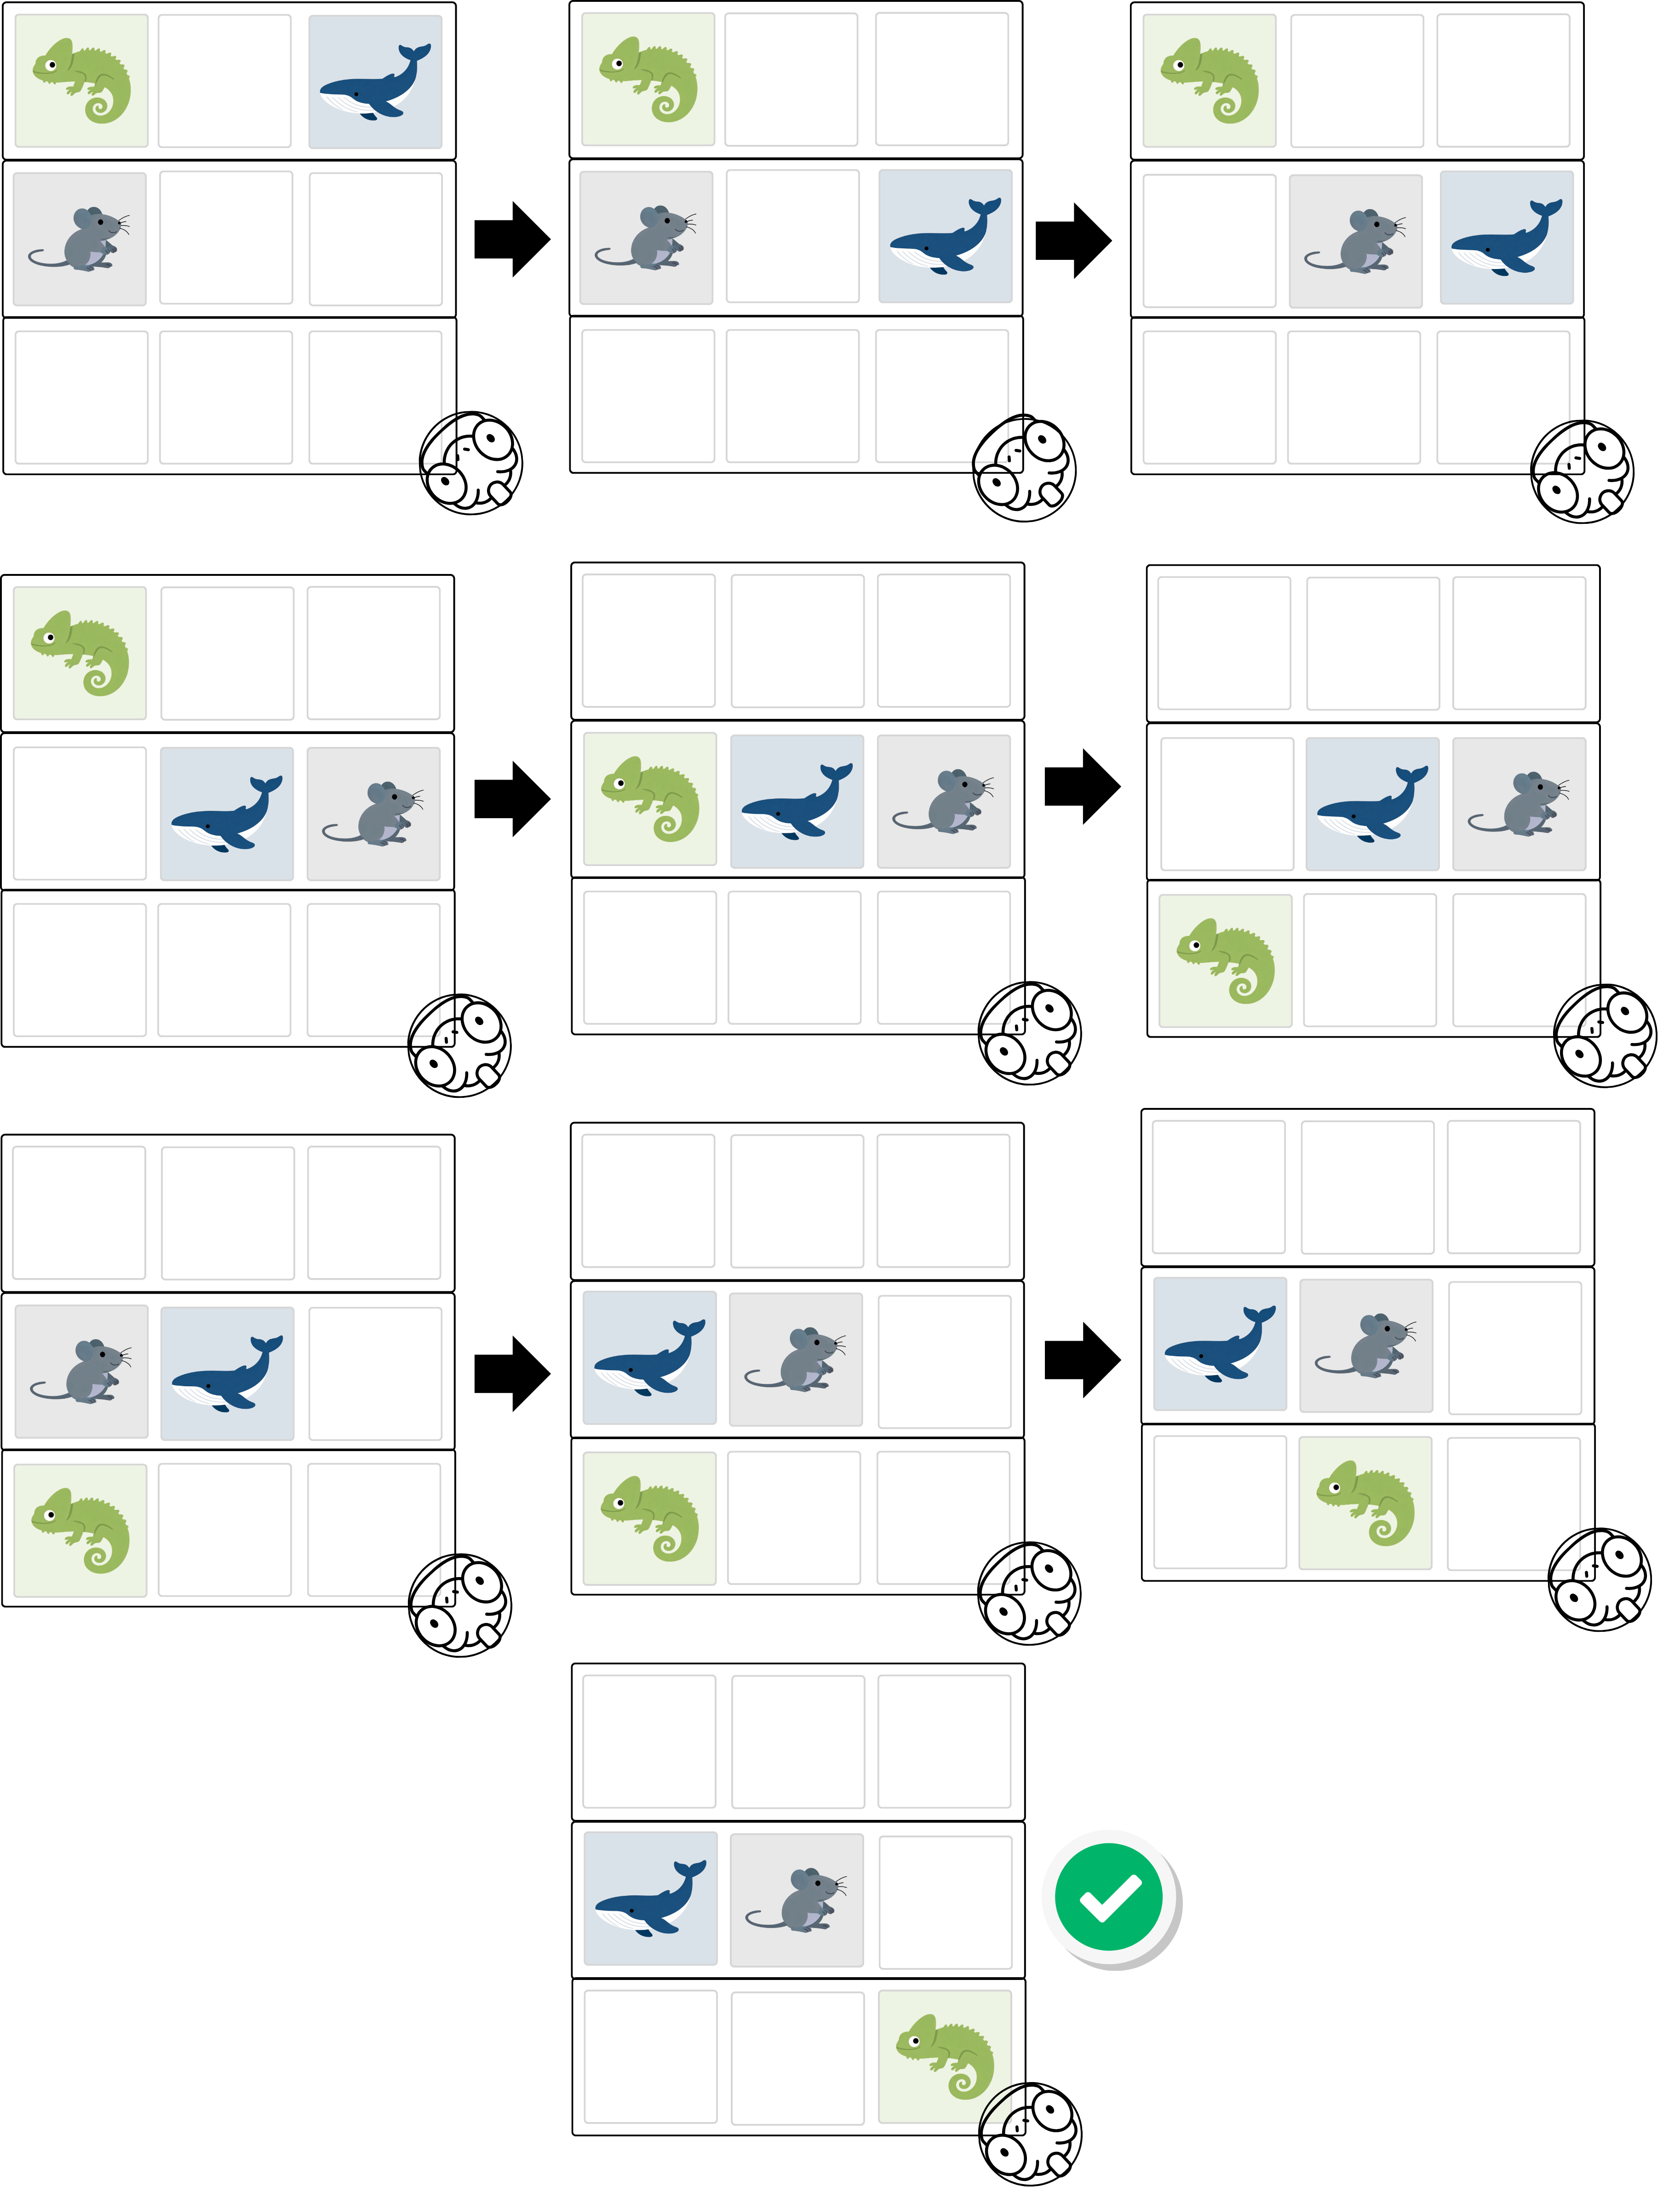
\includegraphics[scale=0.15]{imagens/nivel-aprofundamento-camaleao.png}
    \\\textbf{Fonte:} Elaborado pelo Autor
    \label{fig:rascunho-nivel-aprofundamento-camaleao}
\end{figure}
\FloatBarrier

Aqui não terminei de escrever ainda.

\subsubsection{Coelho}

A peça do Coelho possuirá uma cor branca, contendo o desenho de um coelho. Ao ser clicado, se multiplica para espaços adjacentes vazios. A adjacência, nesse caso, se trata dos espaços acima, abaixo, a esquerda e a direita. O Coelho não empurra nem troca de lugar com outras peças. Caso não haja espaços adjacentes vazios, o Coelho simplesmente desaparece.

\begin{figure}[!htbp]
    \centering
    \caption{Rascunho do Nível Introdutório da Peça Coelho}
    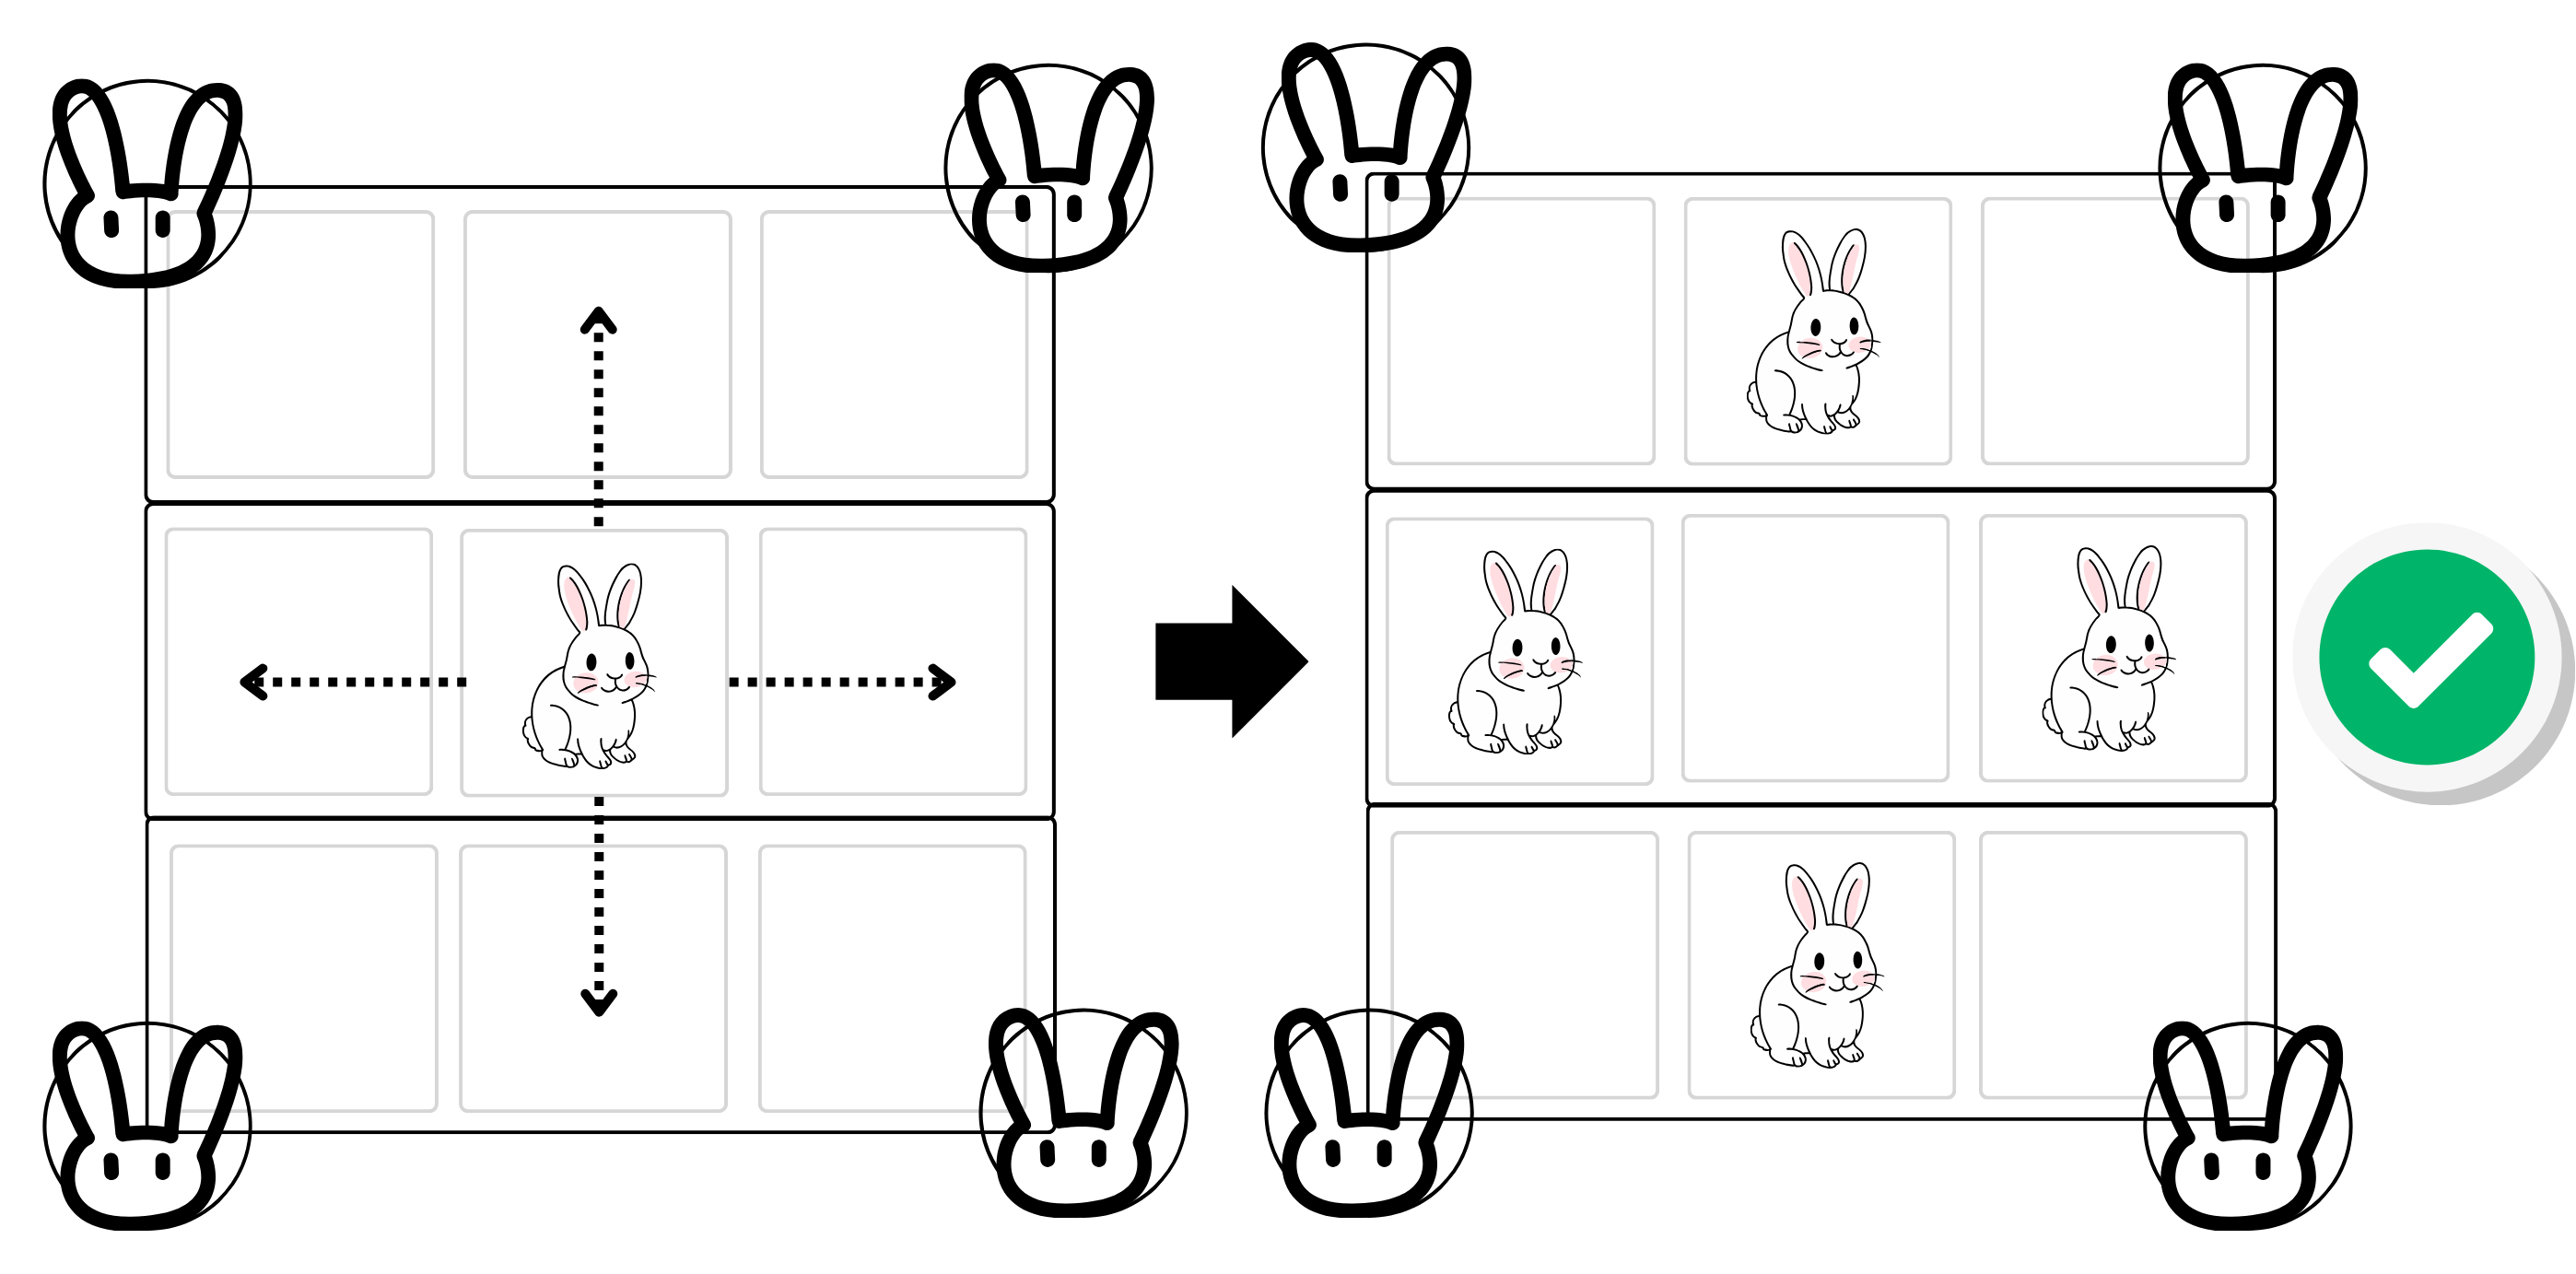
\includegraphics[scale=0.15]{imagens/nivel-introdutorio-coelho.png}
    \\\textbf{Fonte:} Elaborado pelo Autor
    \label{fig:rascunho-nivel-introdutorio-coelho}
\end{figure}
\FloatBarrier

\begin{figure}[!htbp]
    \centering
    \caption{Rascunho do Nível de Aprofundamento da Peça Coelho}
    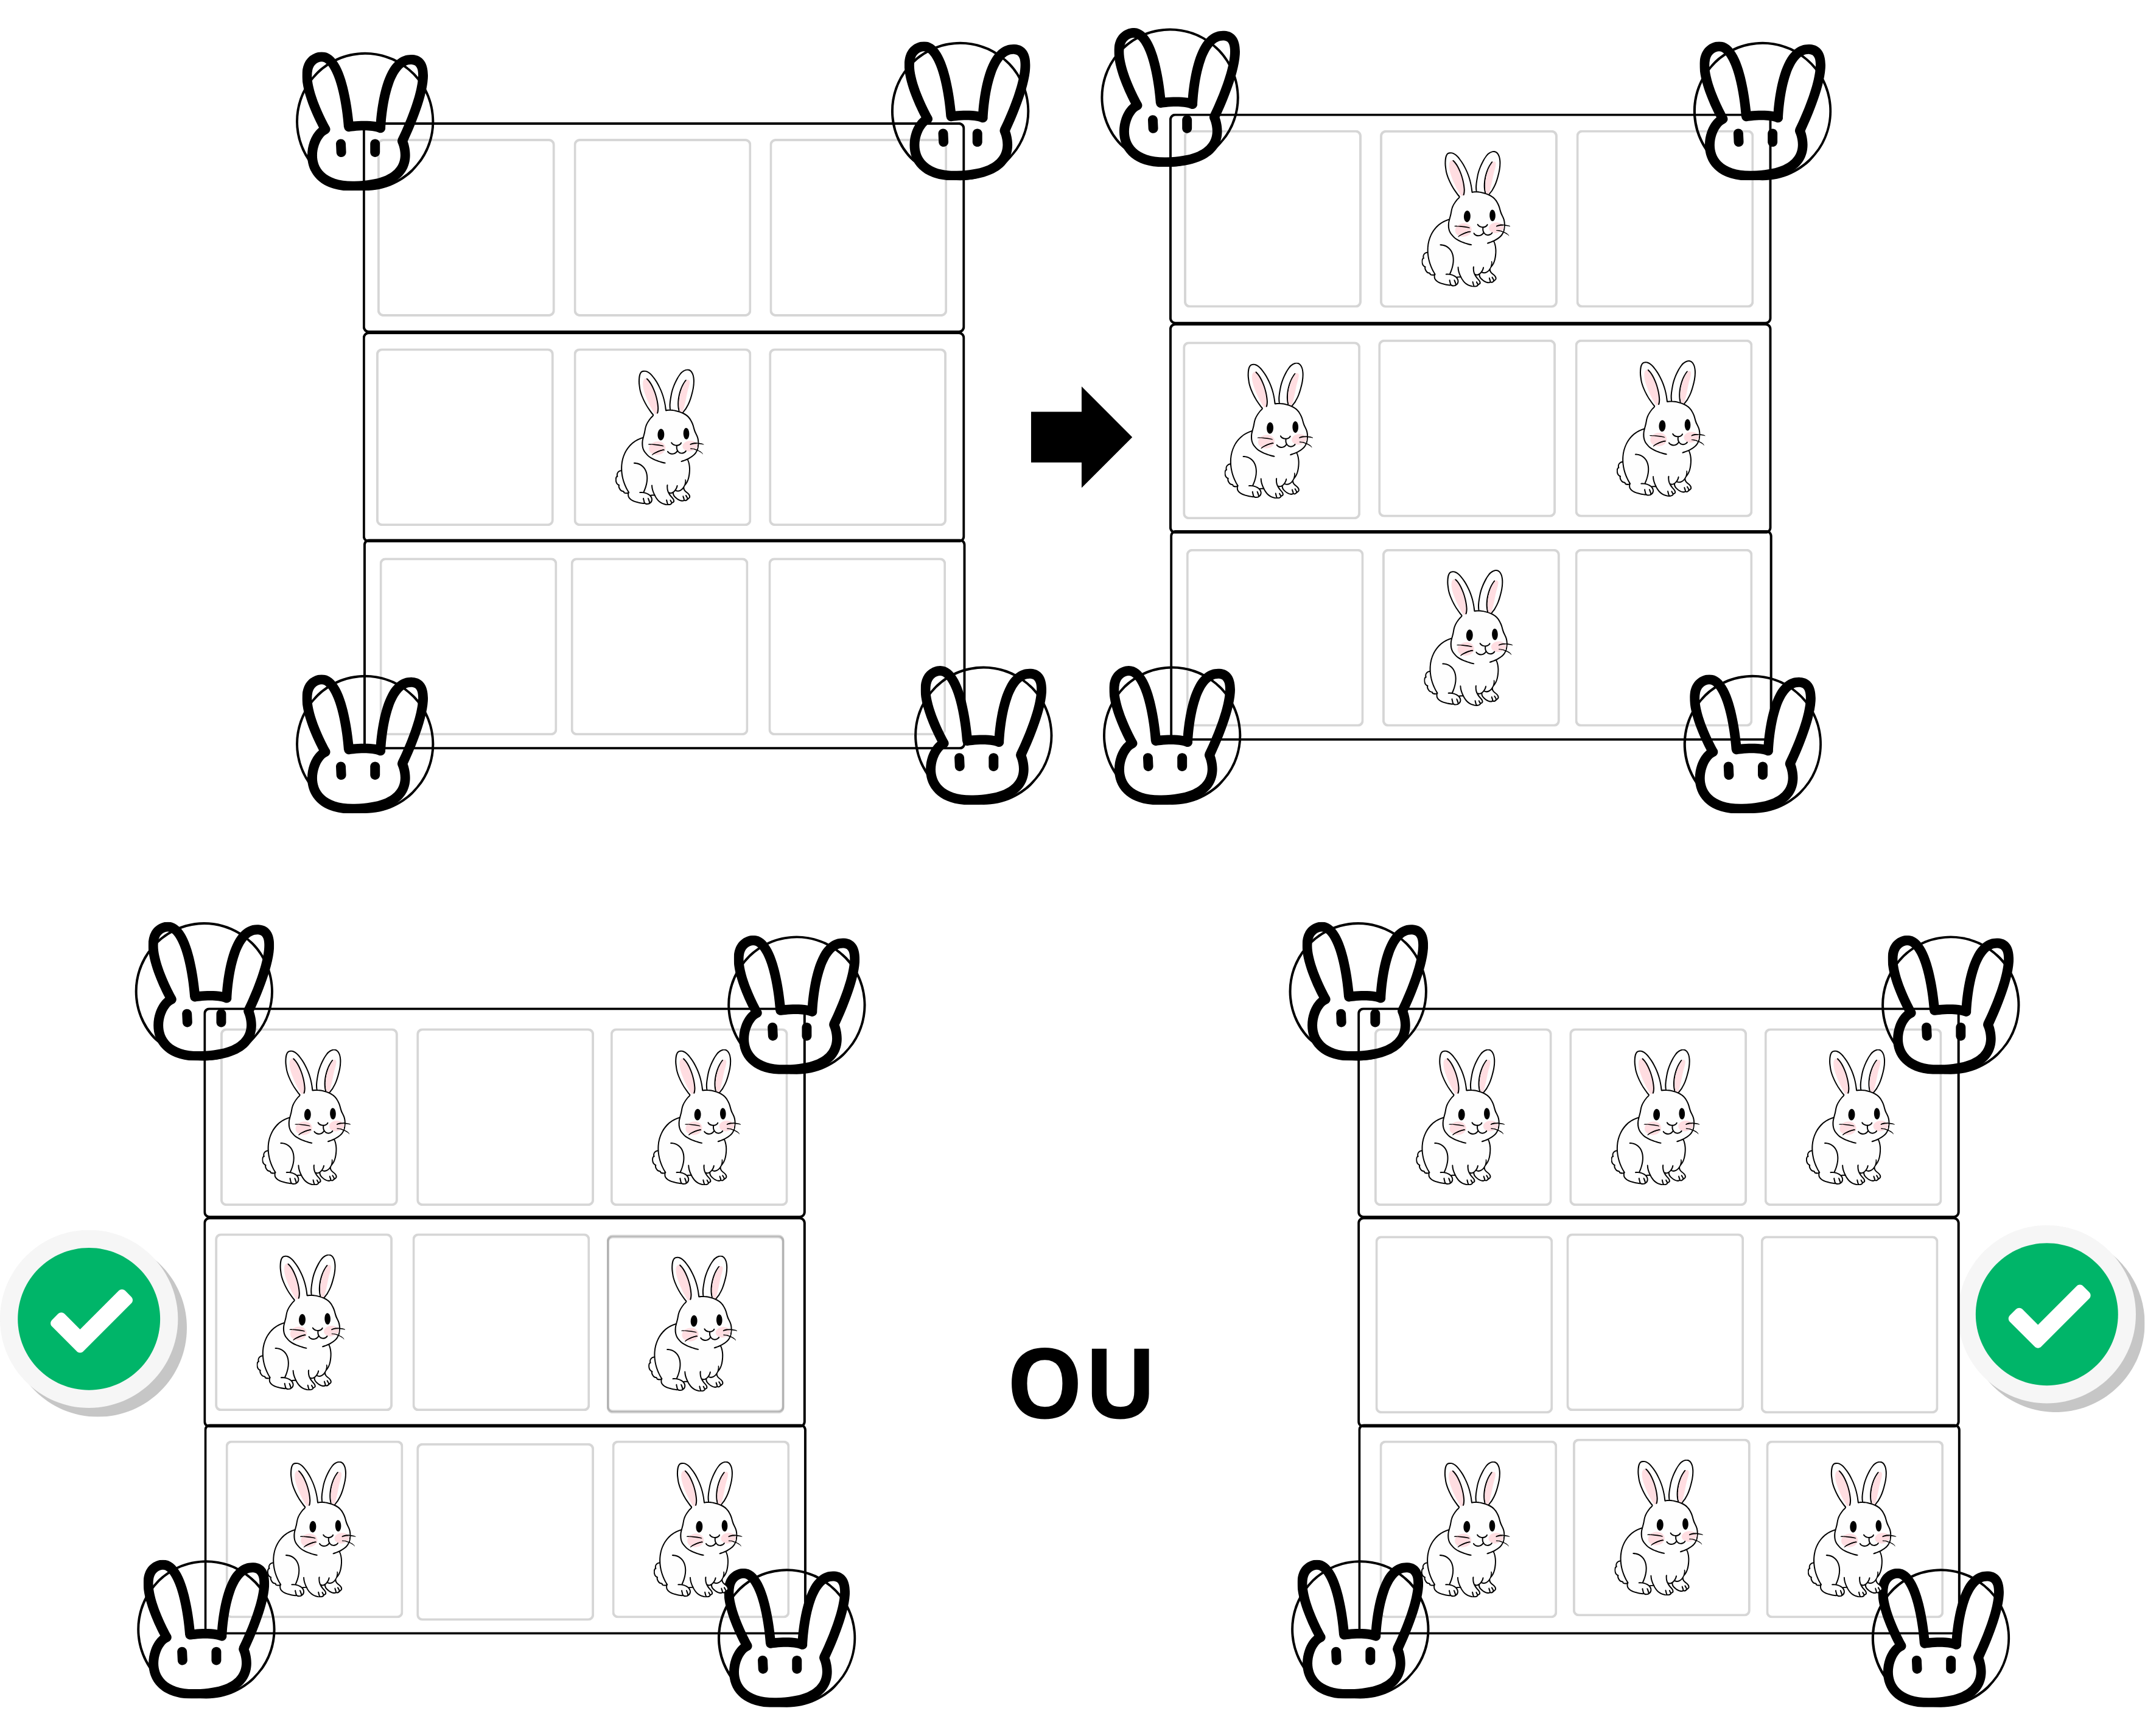
\includegraphics[scale=0.15]{imagens/nivel-aprofundamento-coelho.png}
    \\\textbf{Fonte:} Elaborado pelo Autor
    \label{fig:rascunho-nivel-aprofundamento-coelho}
\end{figure}
\FloatBarrier

Aqui não terminei de escrever ainda.

\subsubsection{Toupeira}

A peça da Toupeira possuirá uma cor acinzentada-escura, contendo o desenho de uma toupeira. Ao ser clicada, a Toupeira teleporta para a posição oposta. Caso esteja em uma das quinas, a Toupeira se teleporta para a diagonal contrária. Ex: caso a Toupeira esteja na diagonal superior da esquerda, ao ser clicada, se teleporta para a diagonal inferior da direita. 

Além do teleporte, a Toupeira também troca de lugar com quaisquer peças que estavam na posição na qual a Toupeira irá ao ser clicada.
Caso a Toupeira esteja no meio do tabuleiro 3 × 3, ela não se teleportará para lugar algum ao ser clicada.

\begin{figure}[!htbp]
    \centering
    \caption{Rascunho do Nível Introdutório da Peça Toupeira}
    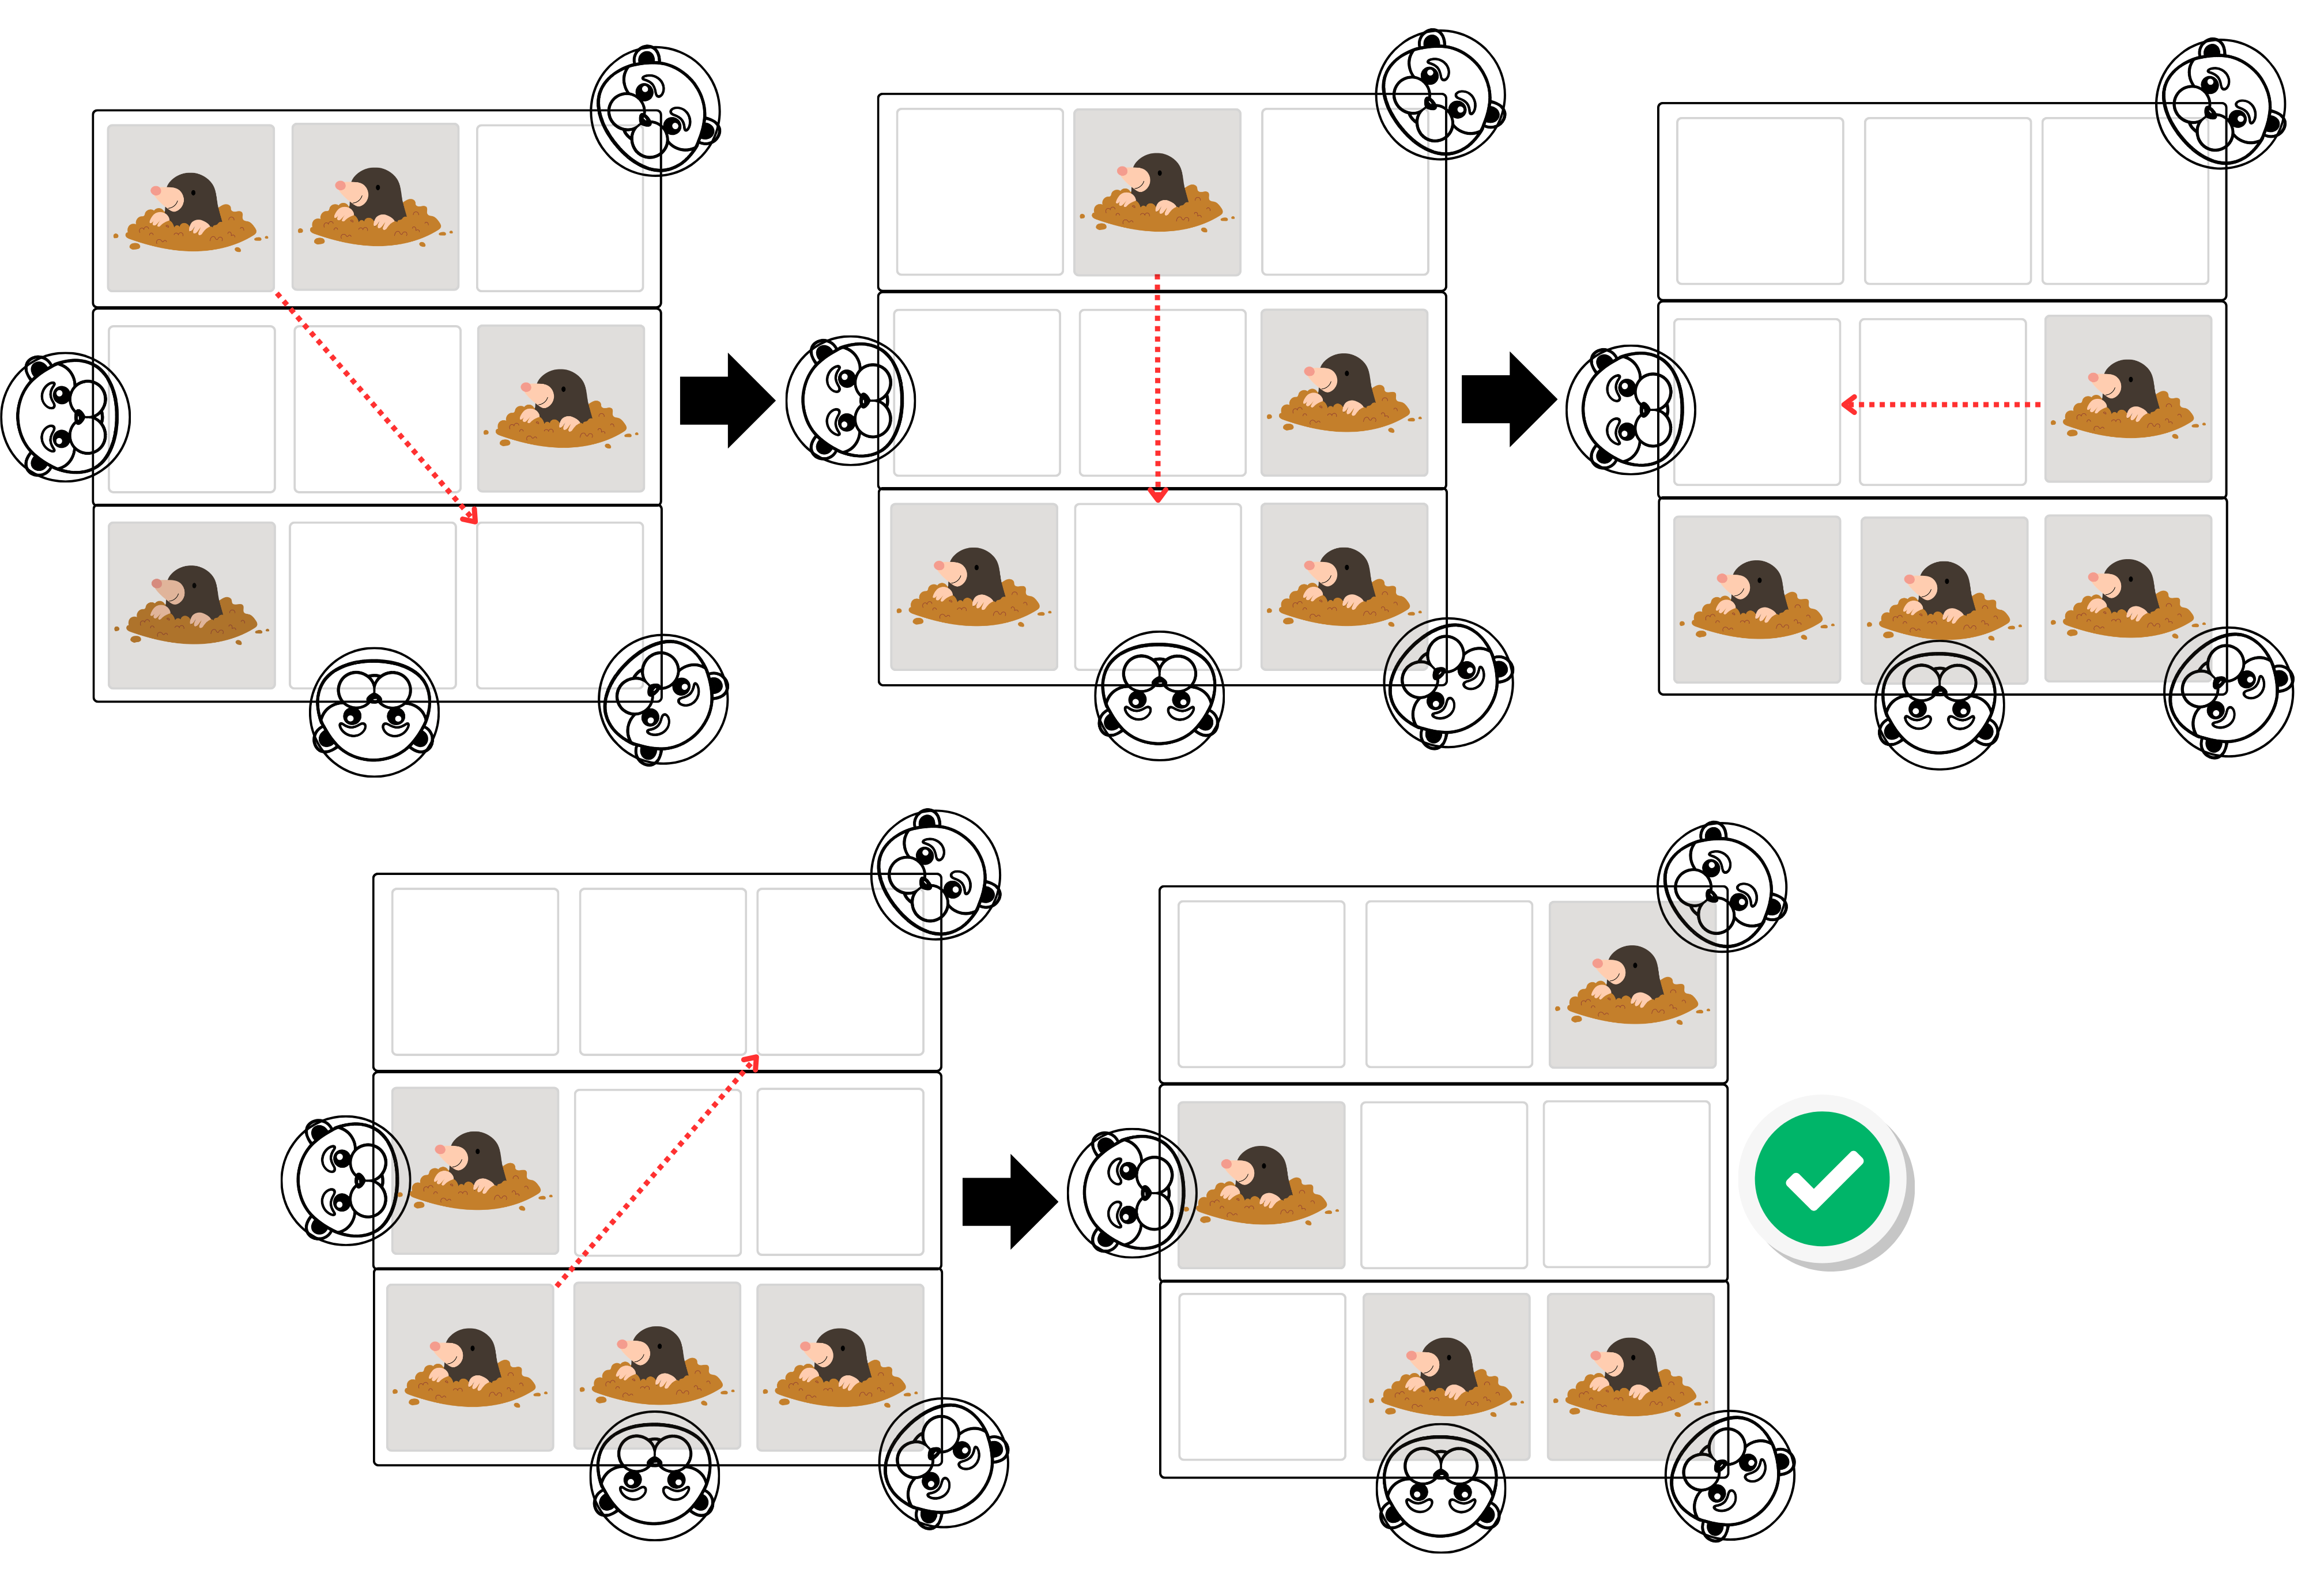
\includegraphics[scale=0.15]{imagens/nivel-introdutorio-toupeira.png}
    \\\textbf{Fonte:} Elaborado pelo Autor
    \label{fig:rascunho-nivel-introdutorio-toupeira}
\end{figure}
\FloatBarrier

Aqui não terminei de escrever ainda. Além disso, não fiz o nível de aprofundamento da toupeira ainda... 

\subsection{Níveis Finais}

não fiz os níveis finais ainda...

\section{Cronograma do Trabalho}

Segue abaixo o cronograma das atividades que serão executadas até a Avaliação Final de TCC.

\FloatBarrier
\begin{figure*}[!htbp]
	\centering
	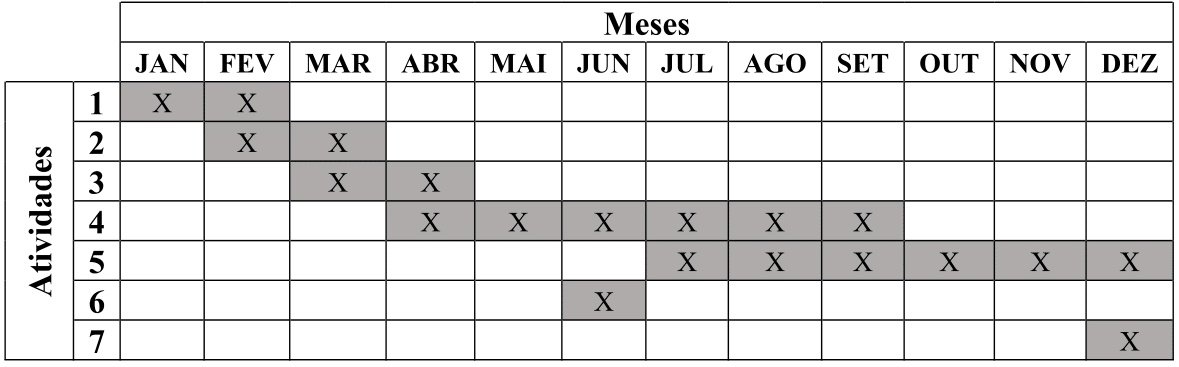
\includegraphics[scale=1]{imagens/cronogramaProjeto.png}
\end{figure*}
\FloatBarrier

\begin{enumerate}
	\item Revisão bibliográfica acerca da IHC e \textit{Design} de Jogos;
	\item Definição das diretrizes e critérios para um bom \textit{Design} de Jogo de \textit{Puzzle};
	\item Planejamento do protótipo;
	\item Desenvolvimento do protótipo com base nas diretrizes;
	\item Testes do Protótipo;
	\item Validação do TCC;
	\item Defesa do TCC.
\end{enumerate}